% T11 of the Transport Papers series.
% Work-order closure (2026-09-13, per Leon, WORK ORDER T13-KNOCKONS item 3).
%   The order recorded that this paper "still records only the routing of the
%   massless locus and successor problems (3) and (4) to T13, where T13's
%   Proposition 4.1 now answers Rem 5.10's question outright". Both sites
%   repaired; no mathematics, label or number changed, no new label added,
%   numbering stays frozen per rule 21, printed version stays 1.0 per rule 25.
%   rem:join (Rem 5.10), closing clause: "whether the condensation
%     programme's seed lies on this locus or in the quantisation of the next
%     remark is a question for the families paper" -> the families paper has
%     since settled it, the seed being the source term, the Lambda-linear
%     tilt of the mass functional, rather than a point of the massless locus,
%     with locator [Props. 4.1-4.2]{ButlerT13} (T13 prop:condensation 4.1,
%     prop:source 4.2, both confirmed against T13's .aux).
%   sec:position, "Papers that rely on this one", T13 entry: the routing
%     sentence now also records that T13 settles Remark 5.10 outright, same
%     locator.
%   Compile: pdflatex x2, 24 pages (unchanged), 0 errors, 0 undefined refs,
%   so T17's status row and verify_T17.py's pages dict need no change.
%   verify_T11.py 39/39. verify_crossrefs.py suite sweep 604/604, 0 skipped,
%   0 broken, both directions (599 before this pass; the 5 added are the new
%   locators here and in T12 and T15). All run in the cloud workspace.
% Correction (2026-09-10, mechanical pass, per Leon): rule 23 misidentified T5 as the printed-version exception. T1 is the exception at Version 3.0; every other paper, T5 included, reads Version 1.0. \date corrected accordingly (was 1.1).
% v1.1 (2026-09-10, derivation session, Fable 5.1 subagent, per rule 20,
%   series-review repair pass against series_review_2026-09-09.md).
%   sec:position, "Papers that rely on this one": the T12 imports listed as
%     T12 actually cites them (Fact 2.1, Thm 3.1 and Cor 3.2, Prop 4.1,
%     Lem 5.1, Def 5.4, Thm 5.6, Prop 5.7) (review 3, internal wording).
%   Bibliography: ButlerT15 subtitle brought to T15's actual title, "The
%     Empty Twistor, the Seesaw Scale, and the Bet at the Floor" (review 2.5).
%   Printed version 1.0 -> 1.1.
%   Script: verify_T11.py 39/39 (docstring version line only; re-run).
%   Compile: pdflatex x2, 24 pages, 0 errors, 0 undefined refs, 0 multiply defined, 0 overfull, no float overflow.
% 2026-09-09 addendum (interactive session with Leon, Opus 5). Two changes
%   per Leon: (1) the printed version is now 1.0 for every paper T0 to T17,
%   T5 alone at 3.0 (progress-doc rule 23); the development numbering is
%   retired from the title page and kept in this header. (2) Every reference
%   to the programme monograph is removed (rule 24), re-pointed to the series
%   where a sibling paper carries the result and otherwise restated to stand
%   alone. No mathematics, no labels and no numbering changed, so verify_T11.py
%   stands unchanged at 39/39 and was not re-run.
%   Here: the two Rem 4.9 citations now point at T6's convention note for the
%   convention rather than for a correction; Position wording follows.
% v1.7 (2026-09-09, derivation session, Fable 5.1 subagent, per rule 20,
%   review-repair pass against T11_review_v7.md, same session; the review of
%   the v1.6 prose pass found no BLOCKING and no SERIOUS items). Fixed the
%   cheap NON-BLOCKING ones: N1 \date updated to 1.7 (was 1.5); N2 the
%   introduction's "proves ..., to compute ..., to say" restored to parallel
%   finite verbs; N3 script label "the mirror grip M(n_0)" -> "the grip on
%   n_0, M(n_0)"; N4 rem:plain "does not confirm the natural conjecture" ->
%   "the natural conjecture fails" (matches rem:hierarchy); N6 rem:gravity's
%   opening clause shortened. Left as recorded: N5 (rem:vacua's contrast, the
%   new sentence judged the more accurate) and N7 (the fact:frozen check is
%   arithmetic on hand-set constants; pre-existing, documents an import).
%   No mathematics, labels, numbering or claims changed. Compiled clean
%   (pdflatex x2, 0 errors, 0 undefined references, 0 overfull boxes, no
%   float overflow, 24pp); verify_T11.py 39/39, set unchanged; numbering
%   frozen: aux diff empty. No knock-ons for other papers noticed.
% v1.6 (2026-09-08, prose pass, Fable 5.1 subagent, per project rule 22:
%   mannered prose replaced by literal statement, Leon's ruling to replace the
%   recurring vocabulary too). Body only; no mathematics, labels, numbering or
%   claims changed. Compiled clean (pdflatex x2, 0 errors, 0 undefined
%   references, 24pp); verify_T11.py 39/39, unchanged; numbering unchanged
%   (aux diff empty). Glossary items applied: "The ledger of levels" heading
%   -> "The levels of the results" (1); "the ledger" / "the pair ledger" in
%   rem:gravity -> "the levels of the results" (1) and "the boundary mode
%   space" (2); "Touchpoint" -> "Point of contact" (4); "verdict" ->
%   "conclusion" (3); "kills" -> "annihilates" (4); "owns" -> "carries" /
%   "contains" (3); "buy" -> "yield" (3, incl. rem:hierarchy title); "grip"
%   as a VERB -> "couple" (4; the noun "the grip" stays, defined object);
%   "joints" -> "steps" (2); "lives in / sits in" -> "lies in / is in" (4);
%   "pinned" -> "fixed"; "from scratch" -> "independently"; "cannot see /
%   sees" -> "insensitive to / affects"; "in disguise" -> "under another
%   name"; "bookkeeping parameter" -> "formal parameter" (2).
%   Non-glossary: "ruler" -> "unit / scale" (4); "sharper coordinates /
%   sharper clothes" -> "restated" (3); "anchor for the sign" -> "reference
%   for the sign"; "single parent" -> "derive from a single object"; "seat of
%   the forces" -> "where the forces arise"; "the tool" -> "the method" (2);
%   "the drop from" -> "the difference between"; "mirror grip" -> "the grip
%   on n_0"; "surprise / triumph / vast / astronomically / cosmically"
%   removed. Abstract trimmed to 250 words (the Tier B gloss dropped).
%   "seed" (T13's condensation seed) and "broken generators" left as names.
% v1.5 (derivation session, 2026-09-03; from T11_review_v5.md, the targeted
%   verification pass on v1.4, which CLEARED the paper subject to V1).
%   Compiled clean (pdflatex x2, 0 errors, 0 undefined references, 0 overfull
%   boxes, 24pp); verify_T11.py 39/39, unchanged. V1: the Higuchi entry
%   corrected to the scalar-series paper, J. Math. Phys. 28 (1987) 1553, and
%   the section locator dropped (not checkable in-suite). V2: the Phi display
%   in prop:casimir's proof set on its own line (the overfull box). V3:
%   cor:series retitled "The weight polynomial and the two series". V4: the
%   v1.4 entry's "No statement's content changed" corrected below to "no
%   result proved in the paper changed".
% v1.4 (derivation session, 2026-09-02, same day; from T11_review_v4.md, the
%   three-agent review of v1.3). Compiled clean (pdflatex x2, 0 errors, 0
%   undefined references, 24pp); verify_T11.py 39/39 (unchanged set; one
%   label reworded: "null, hence simple by Fact 2.3"). No result proved in
%   the paper changed; fact:dixmier's statement did (N1).
%   N1: fact:dixmier restated as a partial list of the two series the paper
%       uses; the universal negative removed; the exceptional series named
%       and declared unused (its scalar members at Delta = 3 + k have
%       m^2 = -k(k+3)H^2, which is where the corollary's w = 1 example sits);
%       Dixmier and Higuchi locators; cor:series(3) reworded to "outside
%       both series used". N2: the Casimir normalisations of fact:dixmier and
%       prop:casimir distinguished in both places. N3: T15 "is routed".
%       N4, N5, N10: tr E^2; Gram indices alpha, alpha', beta, beta';
%       lem:invforms relabelled and cited as Lemma. N6-N9, N11-N15: as
%       listed (Part D sentence split, script sentences made exact, K instead
%       of M in rem:nullity, rem:hierarchy's endpoints, general-n clause in
%       fact:frozen, T9 Prop 4.5(1) added, contribution (3) split, header).
%   Lemma 5.1's proof broken into headed steps with displays.
% v1.3 (derivation session, 2026-09-02, same day; from T11_review_v3.md, the
%   three-agent review of v1.2). Compiled clean (pdflatex x2, 0 errors, 0
%   undefined references, 23pp); verify_T11.py 39/39 exact checks pass
%   (one added: the anti-Hermiticity condition on the x-slot has rank four,
%   so the real slice is the whole real locus; the lem:dsscale(3) check now
%   forms the ambient pairing and tests simplicity; the prop:casimir check
%   now includes the closed form (3)). All findings F1-F25 addressed; no
%   mathematics changed.
%   F1: the ledger lists prop:weight once, under flagged, with its proved
%       half named. F2: fact:chart's in-series locators corrected (T6 Sec 4.2
%       for the flat model, Lem 4.8 for the scale function) and the
%       flat-model dictionary proved in one paragraph inside lem:dsscale(2).
%   F3: lem:real credits T9 Prop 4.5(2) for its first half; eq:hermitian
%       cites T9 Prop 4.5(2),(4); contribution (3) and the ledger say so.
%   F4: rem:sign no longer appeals to an unnamed convention; the BEG sign
%       comparisons in fact:frozen and fact:thomas replaced by T6 Lem 4.8 and
%       two internal anchors (w = 1 returns the frozen point, w = -1 the
%       conformally coupled scalar). F5: NEW fact:dixmier (the unitary
%       classification, imported); cor:series proves the algebra and takes
%       the names from the Fact; ledger aligned. F6: script forms the ambient
%       norm; rem:nullity states the sqrt2 scaling the script uses. F7: real
%       points DEFINED (translation generator in su(2,2)) and shown to be
%       exactly the slice. F8: grading element now E, group elements gamma.
%   F9: Section 8 symbol fixed; Part D opening reworded. F10: Position
%       states what T15 imports, neutrally. F11: five predecessors; T16's
%       import named correctly. F12-F14, F16-F19, F24: as listed (abstract
%       range clause, helicities in rem:join, Dixmier credit unified, Thomas
%       1926 entry, coordinates x^0..x^3 in eq:realslice, epsilon := H/m
%       defined, generic bivector U in lem:chartiso's proof, the tractor
%       bundle symbol dropped, Section 8 wording). F15: q dropped, q(M')
%       in fact:palatial. F20: Lambda != 0 hypotheses added to prop:casimir(3)
%       and prop:weight; four items added to the not-checked list. F21:
%       rem:sign, rem:plain, rem:join in the ledger; rem:nullity in the plan
%       and contribution (3). F22: the figure's glyph is now a double arrow
%       and its caption "One grip, two readings". F23: lem:invforms is now
%       Lemma 2.7 with its proof (Schur imported); T10 cited at Secs 5-6;
%       T6 Prop 4.10 for the group; T9 Thm 4.2(2) credited for -2 det.
%       F25: header wording; script docstring 1.2 -> this version.
%   Fact numbering: Facts 2.1-2.5 unchanged, NEW Fact 2.6 dixmier, Lemma 2.7
%   invforms. Section 5 numbering unchanged from v1.2.
% v1.2 (derivation session, 2026-09-02, same day; from T11_review_v2.md, the
%   three-agent review of v1.1). Compiled clean (pdflatex x2, 0 errors, 0
%   undefined references, 22pp); verify_T11.py 38/38 exact checks pass (six
%   added: universal opposite-sign failure on the grid, shadow symmetry and
%   the general-n conformal weight, the sign of m^2 inside and outside
%   [-3,0], the spanning rank for lem:dsscale(2), su(2,2) membership of the
%   generators of real pairs, the rotation commutator identity, and the
%   reality of the grip).
%   B1: cor:series(3) corrected: real w gives m^2 >= 0 only on [-3,0]; outside,
%       the tachyonic branch. Echoes in the introduction and rem:hierarchy.
%   B2: the real slice of the x-slot corrected to x = (i/sqrt2) K eps
%       (eq:realslice); NEW lem:real proves that the generators of real pairs
%       lie in su(2,2) (translation and special-conformal blocks by direct
%       computation, Lorentz by the rotation commutator identity) and that
%       the grip is a real vector of I-perp, so m^2 is a value of the (1,4)
%       form. The Hermitian form (5.6) is now given its provenance (the
%       standard twistor norm) and declared a chart convention; the
%       index-free pairing (u|v) is written out.
%   B3: rem:gravity: the T5 import removed (T5 says nothing about the
%       graviton); the acoustic no-go stated as T10 states it, on either
%       reading, at the mixed level, one joint conditional. T5 bibitem
%       dropped.
%   S1: framing aligned with the ledger: abstract, introduction, Section 5
%       opening and figure caption no longer say the two formulas are proved
%       to be one number; the flat formula is the squared pairing against I
%       (proved), the de Sitter extension is computed (proved), the composite's
%       weight is read off the dictionary (a definition, prop:weight).
%   S2: prop:casimir restated with the composite and the grip quantified and
%       Greek basis indices; its proof broken into four displayed steps.
%   S3: rem:sign and fact:frozen state what T6 Rem 4.9 says (an inconsistency
%       in the monograph, not a convention). S4: fact:chart cites T9 Thms 3.1
%       and 3.4 and T6 Sec 4.2. S5: Position lists T0, T15, T16; T5 dropped.
%   S6: proof sentences about the script corrected; the tautological
%       conjunct in Part E replaced. S7: "Re w = -3/2" qualified in the
%       introduction and the caption. S8: fact:action transcribes T10 Thm 3.1
%       (defined where the connection is regular). S9: lem:five in the plan
%       and contribution (3); rem:nullity and lem:real in the ledger.
%   Minor: N constituents (not k); Gram scalar q in thm:grip(5); ambient
%       bivectors U, U' in fact:chart; hbar as bookkeeping parameter; the
%       momentum reading of P stated with its n_inf part; lem:five pointer for
%       the SO(1,4) surjection; Tier B glossed; "twice their helicities";
%       Dixmier attribution split; figure cited from Section 4; negations
%       restated positively; T9 Cor 4.8 credited in lem:dsscale(3); the dual
%       metric's self-inverse property shown; 3 x 10^38 throughout; T9
%       realisation named in fact:palatial; successor (5) marked unproved
%       beyond N = 2; Section 8's not-checked list extended.
%   Inbound knock-ons (K1-K9 of T11_review_v2.md) are for the other papers'
%   sessions; the mapping from v1.0 numbering is in the v1.1 entry below.
%   New numbering of Section 5 in this version: Lem 5.1 dsscale, Rem 5.2
%   nullity, Lem 5.3 chartiso, Def 5.4 grip, Lem 5.5 real, Thm 5.6 grip,
%   Prop 5.7 casimir, Lem 5.8 five, Prop 5.9 weight, Rem 5.10 join,
%   Rem 5.11 quantum.
% v1.1 (derivation session, 2026-09-02; from T11_review_v1.md, the fresh
%   three-agent review of v1.0). Compiled clean (pdflatex x2, 0 errors,
%   0 undefined references, 20pp, was 14); verify_T11.py rebuilt, 32/32 exact checks pass.
%   MATHEMATICS.
%   (1) thm:dictionary: the sign corrected. From the paper's own Facts the
%       coupling I.D sigma = 0 gives m^2 = -w(w+n-1)<I,I>, in n = 4
%       m^2 = -w(w+3)Lambda/3 = Delta(3-Delta)H^2 with Delta = -w. v1.0 read
%       the last line of the proof off with the wrong sign and called the
%       result "cleaner than the monograph"; it was wrong. Anchors added as
%       cor:series: the conformally coupled scalar (w = -1) has m^2 = +2H^2;
%       masslessness is w in {0, 1-n}; real weights give m <= 3H/2 (the
%       complementary series); m > 3H/2 forces w = -3/2 +- i nu (the
%       principal series). Facts 2.1 and 2.2 now transcribed in T6's own
%       Schouten convention (P = (Lambda/6) g, J = 2Lambda/3, rho_I = J/n,
%       <I,I> = 2J/n), which v1.0 misreported as BEG's.
%   (2) The exact join rebuilt on the corrected dictionary. The weight
%       equation (old thm:join(2)) is now prop:weight: the composite's weight
%       is w = -3/2 +- i nu with nu = m/H - (9/8)H/m + ..., complex for every
%       known massive particle; the "vast real weights of order 10^38" are
%       imaginary parts. The magnitude heuristic, the (A)/(B) binary and the
%       polynomiality "refutation" (old thm:join(3), prop:closed(2)) are
%       removed: after (1) there was nothing to refute.
%   (3) NEW lem:dsscale: the de Sitter scale in the flat chart, sigma =
%       1 - Lambda Q/12, has scale tractor (sigma, d sigma, -Box sigma/4)
%       parallel with norm Lambda/3; its constant ambient vector is
%       I_Lambda = n_inf + (Lambda/6) n_0. This DERIVES the ansatz, the sign
%       of lambda and the point-supported factor 1 - Lambda Q/12 together
%       (v1.0 assumed the ansatz and appealed to an uncited "stereographic
%       factor of the classical literature").
%   (4) NEW lem:chartiso (the spin isomorphism in the chart, with the
%       translation, special-conformal and grading blocks displayed and
%       proved), def:grip (the moment map, the grip P = M(I) of a composite
%       on the frozen point, m^2 := <P,P>, its SO(1,4)-invariance and flat
%       limit), and thm:grip, the exact join: m^2 = 2|B_Lambda|^2 +
%       <I,I> C with C = (h11-h22)^2/4 + |h12|^2 the internal su(2) Casimir
%       of the Hermitian Gram matrix h_il = conj(Z_i).Z_l. Proved by a
%       printed component computation (three pairings p.p, k.k, p.k - d^2
%       and one determinant identity). The "residue of five constants with
%       one free equation" (old prop:five) is thereby COMPUTED: it is one
%       term, with coefficient exactly <I,I> = H^2. prop:five removed.
%   (5) NEW prop:casimir: <P,P> = <I,I>(C2(so(2,4)) - C2(so(1,4))) and
%       C2(so(2,4)) = tr h^2 - (tr h)^2/4 (proved via lem:invforms and one
%       evaluation on the grading element), so the de Sitter Casimir of the
%       composite is explicit. lem:five keeps the stabiliser count (10/6/5,
%       "six conditions" now stated correctly) and identifies the five
%       broken generators with the grip's components.
%   (6) The mass-floor claim (old rem:buys, abstract) WITHDRAWN: it was
%       false by v1.0's own formulas (aligned point-supported pairs and the
%       doubled composite both have B_Lambda = 0). thm:grip(5) states the
%       exact zero locus instead: m^2 = 0 iff B_Lambda = 0 and h is scalar;
%       the doubled composite has m^2 = H^2 h^2, pure residue, computed.
%   (7) "The chart volume is forced by nullity" WITHDRAWN everywhere:
%       nullity fixes the slot coefficient c = -1/2 once <n_0,n_inf> = 1 and
%       Q = <x,x> are given; it cannot fix a normalisation of the volume
%       form (rem:nullity).
%   PROVENANCE AND HOUSE RULES.
%   fact:chart now sources the bracket and the momentum to Penrose-Rindler
%   and Hughston (T9 has neither), imports the flat-model dictionary
%   (parallel sections = constant vectors, scale function = <X(x),V>) and
%   the identification I = Psi(I_g) from T9 Cor 4.8; fact:palatial drops the
%   "order-one spectra on physical states" clause (not in T9, no longer
%   used) and names q(id), not the normal-ordered charge; fact:action reads
%   "precisely when"; lem:invforms (Humphreys) added. T10 Prop 5.4 cited
%   correctly (nine Goldstone modes, five the I-half). Condensation
%   citations moved from T12 to T13. Position-in-the-series section added
%   (rules 15, 18). Bibliography: T12 entry in house form; T5, T13, T17,
%   Humphreys added. Rule 6: all "fifth refutation" narrative removed (seven
%   sites); the hierarchy statement is neutral. Rule 17a: drafting-history
%   phrases removed; the monograph is referenced only through T6 Rem 4.9.
%   Abstract rewritten (215 words). Figure caption corrected. Date line
%   v1.1. Section 7 rewritten to the 32 checks.
%   A second fresh audit of this version's Section 5 (one agent, before
%   deposit) found a false spanning witness in the proof of lem:dsscale(2)
%   (x = (1,1,0,0) is null and dependent; now x = 2e_0), an unspecified
%   map in thm:grip(4) (now mu_x = -b_x, with the wedge identity proved and
%   scripted), and small over-claims about what the script checks; all
%   fixed. Real slice of the x-slot stated in rem:nullity.
%   KNOCK-ONS FOR OTHER PAPERS (not done here, per rule 20): T12 Fact at its
%   line 126 imports the v1.0 plus-sign dictionary and "N = M_P/H ~ 10^60";
%   T17 rows for refutation 5 and for T11 repeat the withdrawn claims
%   (candidate (A), five constants, 25 checks, 14pp).
%   Inbound locators now stale (verify_crossrefs.py T11 run after this
%   version's .aux was written): T13:100 cites T11 Thm 5.1 and Prop 5.2,
%   T15:97 cites T11 Rem 5.3, T16:100 cites T11 Thm 5.1. Mapping from v1.0:
%   Thm 3.1 and Prop 4.1 unchanged; old Thm 5.1 (the join) -> Thm 5.5
%   (thm:grip), its weight equation -> Prop 5.8 (prop:weight); old Prop 5.2
%   (prop:closed) -> Thm 5.5 and Lem 5.7 (lem:five); old Rem 5.3 (rem:buys,
%   the mass floor) -> Rem 5.9 (rem:join), the floor WITHDRAWN; old Prop 6.1
%   (prop:five) -> computed inside Thm 5.5(2), no separate result; old
%   Rem 6.2 (rem:gravity) -> Rem 6.1. Outbound: 17/17 resolve.
% 2026-08-31 (T6 knock-on, from the re-review of T6 v1.2): rem:sign cited
%   \cite[\S2]{ButlerT6} for the monograph's Theorem 12.6 sign flag, but T6's
%   Section 2 is Setting and conventions and names the monograph nowhere; the
%   flag is T6 Remark 4.9 ("Convention note against the monograph"), and the
%   locator now points there. Content-neutral; no result renumbers.
% 2026-08-24: renumbered (was T16) and retitled per Leon; content unchanged.
% v1.0.1 (sprint 2, 2026-08-21): content-neutral citation repair:
% fact:palatial provenance corrected to T9 Lem 5.5 + Thm 5.7 (was 5.9).
% v1.0 (sprint 2, 2026-08-21): M6: assembly pass; final abstract; one
% rule-13 figure (fig:twolanguages); AWAITING REVIEW.
% v0.5 (sprint 2, 2026-08-21): M5: Machine verification section written;
% verify_T11.py 25/25 exact checks.
% v0.4 (sprint 2, 2026-08-21): M4: Section 6 (prop:five, rem:gravity,
% ledger of levels, five successors).
% v0.3 (sprint 2, 2026-08-21): M3: Section 5 (the exact join: thm:join,
% prop:closed, rem:buys; lambda = +Lambda/6 derived; candidate (A) refuted).
% v0.2 (sprint 2, 2026-08-21): M2: Section 4 (mass as symplectic area,
% prop:area proved, the Fock-vacuum touchpoint).
% v0.1 (sprint 2, 2026-08-21): M1: skeleton, prior art, setting, the
% mass-weight dictionary (Thm 3.1 via the Thomas operator, series
% conventions reconciled: m^2 = +w(w+n-1)<I,I> with <I,I> = Lambda/3).
% House rules: no em dashes; short abstract; standard series disclaimer;
% physics touchpoints kept (rule 10); proof standard per rule 11 (Fact
% (imported) discipline); verification imports GA.py (rule 12); diagrams
% per rule 13; Position in the series (rules 15, 18).
\documentclass[11pt]{article}
\usepackage[margin=1.1in]{geometry}
\usepackage{amsmath,amssymb,amsthm,mathtools}
\usepackage{booktabs}
\usepackage[dvipsnames]{xcolor}
\usepackage{tikz}
\usepackage[colorlinks=true,linkcolor=MidnightBlue,citecolor=MidnightBlue,urlcolor=MidnightBlue]{hyperref}

\newtheorem{theorem}{Theorem}[section]
\newtheorem{proposition}[theorem]{Proposition}
\newtheorem{lemma}[theorem]{Lemma}
\newtheorem{corollary}[theorem]{Corollary}
\theoremstyle{definition}
\newtheorem{definition}[theorem]{Definition}
\newtheorem{remark}[theorem]{Remark}
\newtheorem{example}[theorem]{Example}
\newtheorem{conjecture}[theorem]{Conjecture}
\newtheorem{fact}[theorem]{Fact}
\newtheorem{question}[theorem]{Question}

\newcommand{\R}{\mathbb{R}}
\newcommand{\C}{\mathbb{C}}
\newcommand{\T}{\mathbb{T}}
\newcommand{\tr}{\operatorname{tr}}
\newcommand{\ip}[2]{\langle #1, #2\rangle}
\newcommand{\br}[1]{\langle #1\rangle}
\newcommand{\hp}[2]{( #1 \,|\, #2 )}
\newcommand{\Sc}{\mathbb{S}}

\title{\bfseries The Origin of Mass\\[4pt]
  \large\itshape The Weight Dictionary and the Exact Join}
\author{Leon Butler\\ \normalsize\href{mailto:lbutler.math@gmail.com}{\texttt{lbutler.math@gmail.com}}\\ \normalsize ORCID: \href{https://orcid.org/0009-0006-4449-5617}{0009-0006-4449-5617}}
\date{Version 1.0, September 2026 \textperiodcentered{} Transport Papers, T11}

\begin{document}
\maketitle

\begin{abstract}
\normalsize
Mass enters a conformally invariant theory where scale does: as coupling to the frozen point, the parallel scale tractor of squared norm $\Lambda/3$. We prove the mass-weight dictionary: a density of conformal weight $w$ coupled to the frozen point through the Thomas operator obeys the Klein-Gordon equation with $m^{2} = -w(w+n-1)\ip{I}{I}$, in dimension four $m^{2} = -w(w+3)\Lambda/3$, the de Sitter formula $\Delta(3-\Delta)H^{2}$ with $\Delta = -w$, $H^{2} = \Lambda/3$. A real weight gives a nonnegative $m^{2}$ only on $w \in [-3,0]$, and there at most $m = 3H/2$; every known massive particle has complex weight $-\tfrac32 \pm i\nu$ with $\nu \approx m/H$, about $3 \times 10^{38}$ for the electron. We prove the twistor counterpart, $m^{2} = 2|\br{\pi^{1}\pi^{2}}|^{2}$ for a two-twistor composite, and compute its exact de Sitter extension: the composite's grip on the frozen point, $P = M(I_{\Lambda})$ with $M$ the conformal moment map, is its de Sitter momentum, with squared length
\[
m^{2} \;=\; 2\,|B_{\Lambda}|^{2} + \ip{I_{\Lambda}}{I_{\Lambda}}\, C,
\]
where $B_{\Lambda} = \br{\pi^{1}\pi^{2}} + (\Lambda/6)[\omega^{1}\omega^{2}]$ is the composite's pairing against the frozen point and $C$ the internal $\mathfrak{su}(2)$ Casimir of the constituents' Gram matrix. Relative to the deformed bracket the correction is one term, with coefficient exactly $\Lambda/3$, and the massless locus is computed. The dictionary then assigns the composite its weight; it does not explain the observed masses but relocates the question: the hierarchy is the size of an imaginary weight. The paper is Tier B; every computational identity is verified in exact arithmetic by a deposited script.
\end{abstract}

\medskip
\noindent\textbf{MSC 2020.} Primary 53C80, 81R25; Secondary 53A30, 81T20, 83C60.\\
\textbf{Keywords.} conformal weight; scale tractor; Thomas operator; two-twistor particle; symplectic area; infinity twistor; de Sitter representations; cosmological constant.

\newpage
\textbf{Authorship and disclosure. }The founding idea of the series is the author's: that division by zero in a Clifford algebra should be read not as a prohibition but as a transport into a higher-dimensional algebra, and that the transported division need not be accompanied by an inverse operation. The direction of investigation and the critical review of the results are likewise the author's. The mathematical development and the drafting of the text were carried out in extended collaboration with Claude Fable 5 (Anthropic), an AI system.

\newpage
\section{Introduction}\label{sec:intro}

The action paper of this series builds the internal vector of gravity's MacDowell-Mansouri functional from the completion's frozen point, the parallel scale tractor $I$ whose squared norm is $\Lambda/3$: the Stelle-West vector is $V = X - (3/\Lambda)I$, made from $I$ and the canonical tractor $X$ \cite{ButlerT10}. That is the framework's account of what gravity is. This paper asks what mass is, and finds the same object at the centre of the answer twice: mass is the strength of a field's grip on the frozen point, measured once as a conformal weight read against the frozen point's length, and once as the length of a composite's momentum, which is the composite's grip on the same point. The paper proves each formula at the series' standard, computes the composite's mass in de Sitter space exactly, with the correction to the flat-space formula derived rather than estimated, and says precisely how the two readings meet: the flat formula is the squared pairing of the composite against the frozen point, and the dictionary then assigns the composite its weight.

The results come in three steps. \emph{The dictionary} (Section \ref{sec:dictionary}): a density of conformal weight $w$ coupled to the frozen point through the Thomas operator obeys the Klein-Gordon equation with
\[
m^{2} = -w(w+n-1)\,\ip{I}{I},
\]
in dimension four $m^{2} = -w(w+3)\Lambda/3$. With $H^{2} = \Lambda/3$ and $\Delta = -w$ this is the de Sitter mass formula $m^{2} = \Delta(3-\Delta)H^{2}$, and it carries its own classification: masslessness is $w \in \{0, -3\}$, the conformally coupled scalar $w = -1$ has $m^{2} = 2H^{2}$, a real weight gives $m^{2} \ge 0$ only for $w \in [-3, 0]$ and then $m \le 3H/2$, and every heavier field has complex weight $w = -\tfrac32 \pm i\nu$. Since $3H/2$ is about $10^{-33}\,\mathrm{eV}$, every known massive particle is of the last kind, with $\nu \approx m/H$, about $3 \times 10^{38}$ for the electron. The natural conjecture, that coupling to the frozen point explains the observed masses, fails: what the dictionary yields is the hierarchy problem restated as the size of an imaginary weight. \emph{The area} (Section \ref{sec:area}): a single twistor is massless; a two-twistor composite has $m^{2} = 2|\br{\pi^{1}\pi^{2}}|^{2}$, the squared symplectic area between its constituents' spinor parts. \emph{The join} (Section \ref{sec:join}): the de Sitter scale in the flat conformal chart is $\sigma = 1 - \Lambda Q/12$, and its frozen point in the twistor chart is $I_{\Lambda} = n_{\infty} + (\Lambda/6)\,n_{0}$, derived rather than assumed. The composite's grip on it, the ambient vector $P = M(I_{\Lambda})$ built from the conformal moment map, is the de Sitter momentum, and its squared length is computed in closed form:
\[
m^{2} \;=\; 2\,|B_{\Lambda}|^{2} + \ip{I_{\Lambda}}{I_{\Lambda}}\,C, \qquad B_{\Lambda} = \ip{I_{\Lambda}}{Z^{1}\wedge Z^{2}} = \br{\pi^{1}\pi^{2}} + \tfrac{\Lambda}{6}[\omega^{1}\omega^{2}],
\]
with $C$ the internal $\mathfrak{su}(2)$ Casimir of the two constituents. At $\Lambda = 0$ this is the area formula, now read as the squared pairing of the composite against the frozen point; for $\Lambda \neq 0$ the correction is a single term whose coefficient is the frozen point's norm. The composite's weight is then read off the dictionary: for every composite heavier than $3H/2$, $\mathrm{Re}\,w = -\tfrac32$ and $\mathrm{Im}\,w = m/H - \tfrac98 H/m + O((H/m)^{3})$. Section \ref{sec:gravity} assembles the results with the action paper, at declared levels: mass is coupling to the frozen point, gravity is the action of the frozen point, and the universality of free fall reads as the statement that the theory contains one scale-giving object.

\subsection*{Prior art}

The tractor calculus and the Thomas operator are Thomas's, in the modern formulation of Bailey, Eastwood and Gover \cite{BEG1994}; the scale tractor and the almost-Einstein technology are Gover's \cite{Gover2010}; the identification of the parallel scale tractor with this series' frozen point, and the norm $\ip{I}{I} = \Lambda/3$ in the series' conventions, are the geometry paper's \cite{ButlerT6}. The two-twistor description of massive particles is classical twistor theory: Penrose, Hughston, and the Oxford school \cite{PenroseRindler1986, Hughston1979}; the mass formula as a two-index contraction with the infinity twistor is standard there, as is the conformal moment map in twistor variables. The three series of unitary representations of $SO(1,4)$ are Dixmier's \cite{Dixmier1961}; the mass formula $\Delta(3-\Delta)H^{2}$ is their modern parametrisation, standard in the de Sitter literature. The identification of the ambient space with $\Lambda^{2}\T$, of the incidence chart with the completion, and of the frozen point with the infinity twistor, which the join relies on, is the twistor paper's \cite{ButlerT9}. What this paper claims as new is the dictionary read through the frozen point, so that mass and dark energy derive from a single object; the derivation of the de Sitter frozen point $I_{\Lambda}$ and its deformed bracket from the scale function of the flat chart; the closed-form mass of the two-twistor composite in de Sitter space, with the correction to the flat formula computed as one term; and the reading of the equivalence principle that the assembly with the action paper permits.

\subsection*{Contribution}

(1) The mass-weight dictionary at theorem level in the series' conventions, with its three de Sitter series as a corollary (Section \ref{sec:dictionary}). (2) The two-twistor area formula, classical, reproved at theorem level because the join needs every sign, with the Fock-vacuum reading from the twistor paper (Section \ref{sec:area}). (3) The exact join: the de Sitter scale and frozen point in the flat chart, what the chart's nullity fixes and the real slice, the chart form of the spin isomorphism, the grip of a composite on the frozen point and its reality (the first half of the reality lemma being the chart form of a twistor-paper statement, the second this paper's), the closed-form mass with its one-term correction, the Casimir form of the result, the five broken generators, and the weight of a composite (Section \ref{sec:join}). (4) The assembly with the action paper at declared levels, and the successor problems (Section \ref{sec:gravity}). (5) Machine verification of every computational identity in exact arithmetic \cite{ButlerVerifyT11}.

\section{Setting and imports}\label{sec:setting}

Notation follows the geometry and action papers \cite{ButlerT6, ButlerT10}: spacetime signature $(+,-,-,-)$, dimension $n = 4$ except where $n$ is displayed, ambient (tractor) bundle of rank six with fibre metric of signature $(2,4)$, and units $G = c = 1$; $\hbar$ is kept as a formal parameter where quantisation is discussed and set to $1$ elsewhere. In a scale $g$ the tractor splits as $V = (\sigma, \mu_{a}, \rho)$ with
\begin{equation}\label{eq:tractormetric}
\ip{(\sigma,\mu,\rho)}{(\sigma',\mu',\rho')} = \sigma\rho' + \rho\sigma' + g(\mu,\mu'),
\end{equation}
the hyperbolic pair on the outer slots and the spacetime metric on the middle. The Schouten tensor is $P_{ab}$, its trace $J = g^{ab}P_{ab}$, and $\Box = g^{ab}\nabla_{a}\nabla_{b}$ is the wave operator, so that the Klein-Gordon equation for mass $m$ reads $(\Box + m^{2})\sigma = 0$. Throughout, $H^{2} := \Lambda/3$, so that $\ip{I}{I} = H^{2}$ for the frozen point below; $H$ is the Hubble rate of the de Sitter background, and ``Hubble units'' means $H = 1$.

\begin{fact}[imported: the frozen point and the tractor connection]\label{fact:frozen}
The ambient bundle carries the canonical connection, whose expression in the scale $g$ is
\begin{equation}\label{eq:tractorconn}
\nabla_{a}(\sigma, \mu_{b}, \rho) = \bigl(\nabla_{a}\sigma - \mu_{a},\;\; \nabla_{a}\mu_{b} + g_{ab}\,\rho - P_{ab}\,\sigma,\;\; \nabla_{a}\rho + P_{a}{}^{b}\mu_{b}\bigr),
\end{equation}
and it preserves \eqref{eq:tractormetric}. On a vacuum Einstein background with cosmological constant $\Lambda$, in these conventions $P_{ab} = (\Lambda/6)\,g_{ab}$ and $J = 2\Lambda/3$, the bundle carries a distinguished parallel section $I$, the frozen point: in its own scale $I = (1, 0, \rho_{I})$ with vanishing middle slot, $\nabla I = 0$ is equivalent to the vacuum equations, and
\[
\rho_{I} = \frac{J}{n} = \frac{\Lambda}{6}, \qquad \ip{I}{I} = \frac{2J}{n} = \frac{\Lambda}{3}.
\]
(The geometry paper is four-dimensional; the general-$n$ form of $\rho_{I}$ is the middle slot of \eqref{eq:tractorconn} for the section $(1, 0, \rho_{I})$, $g_{ab}\rho_{I} = P_{ab}$, traced.) $I$ is null exactly when $\Lambda = 0$; for $\Lambda > 0$ its stabiliser is $SO(1,4)$ and the induced form on $I^{\perp}$ has signature $(1,4)$. \emph{Provenance:} \cite[Fact~4.1, Prop.~4.4, Thm.~4.5, Thm.~4.7, Prop.~4.10]{ButlerT6} (Prop.~4.4 for the stabiliser algebra and the signature of $I^{\perp}$, Prop.~4.10 for the group). The sign of the norm is the series' convention, fixed there and machine-verified; \cite[Rem.~4.9]{ButlerT6} records why that sign is not free: a norm of the opposite sign could not carry the de Sitter stabiliser the same paper establishes. The relative sign of the Schouten slots in \eqref{eq:tractorconn} against the literature is convention-dependent and is fixed internally in the geometry paper \cite[Lem.~4.8]{ButlerT6}; every formula of this paper is written in the convention of \eqref{eq:tractorconn}.
\end{fact}

\begin{fact}[imported: the Thomas operator]\label{fact:thomas}
On a density $\sigma$ of conformal weight $w$ the Thomas operator $D$ produces the tractor
\[
D\sigma = \bigl(\, w(n+2w-2)\,\sigma,\;\; (n+2w-2)\,\nabla_{a}\sigma,\;\; -(\Box\sigma - wJ\sigma)\,\bigr)
\]
in the splitting of a scale $g$, and $D\sigma$ is conformally invariant as a weight-$(w-1)$ tractor field. For $w = 1$ and a scale $\sigma$, $\tfrac1n D\sigma$ is the scale tractor of $\sigma$, whose parallelism is the Einstein condition of Fact \ref{fact:frozen}. \emph{Provenance:} Thomas's prolongation \cite{Thomas1926}, in the form of \cite{BEG1994}; see also \cite{Gover2010}. The sign of the $J$-term follows the sign of the Schouten tensor in the connection, and within the convention of \eqref{eq:tractorconn} it is the one displayed: at $w = 1$ on the constant density $1$ of an Einstein scale the display returns $(1, 0, J/4) = (1, 0, \Lambda/6)$, the frozen point of Fact \ref{fact:frozen}, a consistency the paper's own computations confirm (Lemma \ref{lem:dsscale}(1), Corollary \ref{cor:series}(2)). No translation between conventions is used.
\end{fact}

\begin{fact}[imported: the flat model, the twistor chart, and the infinity twistor]\label{fact:chart}
On a conformally flat region the ambient bundle is trivial: its fibre is one fixed vector space $V$ with the ambient pairing, parallel sections are constant vectors, and the canonical tractor at the point $x$ is $X(x) = n_{0} + x - \tfrac12 Q(x)\, n_{\infty}$, with $n_{0}, n_{\infty}$ null, $\ip{n_{0}}{n_{\infty}} = +1$, $x$ in their orthogonal complement, and $Q(x) = \ip{x}{x} = g(x,x)$ the flat quadratic form, so that $\ip{X(x)}{X(x)} = 0$ identically. The scale function of a constant vector $V$ is its $\sigma$-slot in the flat scale, $\sigma_{V}(x) = \ip{X(x)}{V}$. The complexification of $V$ is $\Lambda^{2}\T$ for $\T$ the twistor space (the chirality half of the ascended Dirac module), with pairing $\ip{U}{U'} = \varepsilon(U \wedge U')$ for the volume form $\varepsilon$ on $\Lambda^{4}\T$ that the identification fixes; a bivector is simple iff its norm vanishes; the mixed slot carries $\ip{x}{x} = -2\det x$ in the chart's components \cite[Thm.~4.2(2)]{ButlerT9}; a twistor splits as $Z = (\omega, \pi)$ with $\omega$ in the two-plane $\Sc$ whose Pl\"ucker bivector is $n_{\infty}$ and $\pi$ in the two-plane $\Sc'$ whose Pl\"ucker bivector is $n_{0}$. The action of $\mathfrak{sl}(\T)$ on $\Lambda^{2}\T$ by $A\cdot(u \wedge v) = Au \wedge v + u \wedge Av$ is a Lie algebra isomorphism onto $\mathfrak{so}(\Lambda^{2}\T, \varepsilon)$, and the infinity twistor of a scale is the image of its scale tractor: for a vacuum with $\Lambda = 0$ it is covariantly constant and simple, the Pl\"ucker bivector of the infinity line. \emph{Provenance:} the flat model as a fixed vector space with the point embedding is \cite[\S4.2]{ButlerT6}, the scale function $\sigma = \ip{X}{I}$ recovering $g = \sigma^{-2}\eta$ is used in \cite[Lem.~4.8]{ButlerT6}, and the general form of the dictionary (parallel sections are constant vectors, with $\sigma$-slot $\ip{X(x)}{V}$) is \cite[\S2]{BEG1994}; in the form needed here it is elementary and is proved in one paragraph inside Lemma \ref{lem:dsscale}; the chirality half is \cite[Thm.~3.1]{ButlerT9}; the identification $V_{\C} = \Lambda^{2}\T$ with its pairing, the normalisation of $\varepsilon$, the simplicity criterion, and the equivariance of the identification are \cite[Thm.~3.4]{ButlerT9}; the chart, the identification of the incidence relation with the completion's own chart, the spin isomorphism, and the infinity twistor are \cite[Thm.~4.2, Cor.~4.8, Prop.~5.2]{ButlerT9}, in that paper's sign conventions, machine-verified there. The spinor bracket $\br{\pi^{1}\pi^{2}} = \varepsilon^{AB}\pi^{1}_{A}\pi^{2}_{B}$, the null momentum $p_{AA'} = \pi_{A}\bar\pi_{A'}$ of a twistor, and the conformal generators as Hermitian quadratics $\bar{Z}_{\alpha}Z^{\beta}$ in the twistor variables are classical \cite{PenroseRindler1986, Hughston1979}.
\end{fact}

\begin{fact}[imported: the palatial quadratics and the homogeneity charge]\label{fact:palatial}
The symmetrised quadratics $q(M)$ in the twistor oscillators represent $\mathfrak{su}(2,2)$ with $[q(M), q(M')] = \hbar\, q([M,M'])$, and, in that paper's realisation $\bar{Z}_{\beta} = -\hbar\partial_{\beta}$, the symmetrised identity quadratic $q(\mathrm{id})$ acts on functions of homogeneity $h$ as $-(h+2)\hbar$ (Penrose's $-2s-2$, proved in the series as an exact identity in the proof of that theorem); the lemma represents all of $\mathfrak{gl}(4,\C)$, of which $\mathfrak{su}(2,2)$ is the real form used here. \emph{Provenance:} \cite[Lem.~5.5, Thm.~5.7]{ButlerT9}. Used here only in Remark \ref{rem:quantum}, to place the classical computation of Section \ref{sec:join} against its quantisation.
\end{fact}

\begin{fact}[imported: the action of the frozen point]\label{fact:action}
Gravity's action is the MacDowell-Mansouri functional of the frozen point: the Stelle-West internal vector is $V = X - (3/\Lambda)I$, made from the frozen point $I$ and the canonical tractor $X$; the functional is polynomial in its arguments and its integrand is defined wherever the ambient bundle and its connection are regular, the field equations reaching the singular locus as conditions on the residue; and its curvature-squared presentation exists precisely when $\Lambda \neq 0$, a boundary of the presentation and not of the action principle. The action clause of that theorem rests on the MacDowell-Mansouri variational identity, imported there at assembly level. \emph{Provenance:} \cite[Thm.~3.1]{ButlerT10}; used here only in the assembly of Section \ref{sec:gravity}.
\end{fact}

\begin{fact}[imported: the unitary representations of the de Sitter group]\label{fact:dixmier}
Among the unitary irreducible representations of $SO(1,4)$ carried by scalar fields, with the Casimir normalised so that it acts as $-m^{2}/H^{2}$ and $m^{2} = \Delta(3-\Delta)H^{2}$, are: the principal series, $m^{2} \ge \tfrac94 H^{2}$, parametrised by $\Delta = \tfrac32 + i\nu$ with $m^{2} = (\tfrac94 + \nu^{2})H^{2}$; the complementary series, $0 < m^{2} < \tfrac94 H^{2}$, with $\Delta$ real in $(0,3)$; and the massless point $m = 0$. No representation of the principal or complementary series has $m^{2} < 0$; the exceptional (discrete) series, which also contains scalar members at $\Delta = 3 + k$, $k = 1, 2, \dots$, with $m^{2} = -k(k+3)H^{2}$, is not used in this paper. \emph{Provenance:} the classification of the unitary representations is Dixmier's \cite[\S\S3--4]{Dixmier1961}; the $\Delta$-parametrisation and the mass formula for the scalar series of $SO(N,1)$ are the modern presentation, for which see \cite{Higuchi1987}. The Casimir normalisation here is the field-theoretic one on a scalar module and is not the $C_{2}$ of Proposition \ref{prop:casimir}, which is the quadratic form on the moment components of a composite; the two differ by the composite's conformal Casimir (Proposition \ref{prop:casimir}(1)). Used to read Corollary \ref{cor:series}, which proves the algebra of $-w(w+3)$ and imports the names of the series from here.
\end{fact}

\begin{lemma}[Invariant forms on a simple Lie algebra]\label{lem:invforms}
On a finite-dimensional simple Lie algebra over $\C$, any two nonzero invariant symmetric bilinear forms are proportional.
\end{lemma}

\begin{proof}
Let $B_{1}$ be the Killing form, nondegenerate by Cartan's criterion \cite[\S5.1]{Humphreys1972}, and $B_{2}$ invariant. Then $B_{2}(A, \cdot) = B_{1}(\phi A, \cdot)$ defines a linear $\phi$, and invariance of both forms makes $\phi$ commute with the adjoint action; the adjoint representation of a simple algebra is irreducible, so $\phi$ is a scalar by Schur's lemma \cite[\S6.1]{Humphreys1972}. Used in Proposition \ref{prop:casimir}.
\end{proof}

\section{The mass-weight dictionary}\label{sec:dictionary}

\begin{theorem}[The mass-weight dictionary]\label{thm:dictionary}
Let $\sigma$ be a density of conformal weight $w$ on a vacuum Einstein background with frozen point $I$, and impose the coupling
\[
I \cdot D\sigma = 0.
\]
Then, in the scale of $I$, $\sigma$ obeys the Klein-Gordon equation $(\Box + m^{2})\sigma = 0$ with
\begin{equation}\label{eq:dictionary}
m^{2} = -\,w(w+n-1)\,\ip{I}{I}, \qquad\text{in } n = 4:\quad m^{2} = -\,w(w+3)\,\frac{\Lambda}{3} = -\,w(w+3)\,H^{2}.
\end{equation}
The mass of a field is its conformal weight, read in the units the frozen point provides, and every mass in the theory is $\sqrt{\Lambda}$ times a factor fixed by the weight.
\end{theorem}

\begin{proof}
Pair $I = (1, 0, \rho_{I})$ with $D\sigma$ in the metric \eqref{eq:tractormetric}. The middle slots contribute nothing since $I$ has $\mu = 0$, leaving the two hyperbolic cross terms:
\[
I \cdot D\sigma = 1 \cdot \bigl(-(\Box\sigma - wJ\sigma)\bigr) + \rho_{I} \cdot w(n+2w-2)\,\sigma .
\]
Substituting $\rho_{I} = J/n$ from Fact \ref{fact:frozen} and collecting the $\sigma$-terms:
\[
I \cdot D\sigma = -\Box\sigma + wJ\sigma + \frac{J}{n}\,w(n+2w-2)\,\sigma
= -\Box\sigma + \frac{wJ}{n}\bigl[n + (n+2w-2)\bigr]\sigma
= -\Box\sigma + \frac{2wJ}{n}(n+w-1)\,\sigma .
\]
Setting this to zero gives $\Box\sigma = \tfrac{2wJ}{n}(n+w-1)\,\sigma$, that is $(\Box + m^{2})\sigma = 0$ with
\[
m^{2} = -\frac{2J}{n}\,w(n+w-1) = -\,w(w+n-1)\,\ip{I}{I},
\]
the last step by $\ip{I}{I} = 2J/n$ (Fact \ref{fact:frozen}). In $n = 4$ with $J = 2\Lambda/3$: $m^{2} = -w(w+3)\Lambda/3$. The script forms the pairing slot by slot from the two Facts, with $\sigma$ and $\Box\sigma$ as formal coordinates, and reads $m^{2}$ off the resulting Klein-Gordon equation, on a rational grid in $(w, n, J)$ and as an identity of rational functions in a formal $\Lambda$; as a consequence, the opposite sign fails the same pairing wherever $m^{2} \neq 0$, which the script also records.
\end{proof}

\begin{corollary}[The weight polynomial and the two series]\label{cor:series}
In $n = 4$, with $\Delta := -w$ and $H^{2} = \Lambda/3 > 0$, the dictionary reads $m^{2} = \Delta(3-\Delta)H^{2}$, the de Sitter mass formula of Fact \ref{fact:dixmier}, whose two series are named below by that Fact; what is proved here is the algebra of $-w(w+3)$:
\begin{enumerate}
\item $m = 0$ exactly for $w \in \{0, -3\}$, the shadow pair $w \leftrightarrow -3-w$ preserving $m^{2}$;
\item the conformally coupled scalar $w = 1 - n/2 = -1$ has $m^{2} = 2H^{2}$; in general dimension $w = 1 - n/2$ gives $m^{2} = \tfrac{n(n-2)}{4}\ip{I}{I}$;
\item for real $w$, $m^{2} = \bigl[\tfrac94 - (w + \tfrac32)^{2}\bigr]H^{2} \le \tfrac94 H^{2}$, with equality at $w = -\tfrac32$; $m^{2} \ge 0$ exactly for $w \in [-3, 0]$, where $m$ runs over $[0, 3H/2]$, the complementary series $0 < m < 3H/2$ together with its two endpoints (the massless pair and the $\nu = 0$ member of the principal series); a real weight outside $[-3,0]$ gives $m^{2} < 0$, outside both series of Fact \ref{fact:dixmier} that this paper uses;
\item for $m > 3H/2$ the weight is complex,
\begin{equation}\label{eq:principal}
w = -\frac32 \pm i\nu, \qquad \nu = \sqrt{\frac{m^{2}}{H^{2}} - \frac94}, \qquad \nu = \frac{m}{H} - \frac98\,\frac{H}{m} + O\!\Bigl(\frac{H^{3}}{m^{3}}\Bigr),
\end{equation}
the principal series: the real part is universal and the mass lies in the imaginary part.
\end{enumerate}
\end{corollary}

\begin{proof}
(1) $w(w+3) = 0$ iff $w \in \{0,-3\}$, and $w(w+3)$ is invariant under $w \mapsto -3-w$. (2) At $w = 1 - n/2$, $w + n - 1 = n/2$ and $-w(w+n-1) = (n/2)(n/2 - 1) = n(n-2)/4$; for $n = 4$ this is $2$. Directly from the operator: at this weight the top two slots of $D\sigma$ vanish, $I \cdot D\sigma = -(\Box\sigma - wJ\sigma) = -(\Box\sigma + J\sigma)$, and $J = 2\Lambda/3$ gives $m^{2} = 2\Lambda/3$, which is the classical value of the conformal coupling $\tfrac16 R$ on de Sitter space in these conventions; this is the convention-independent reference for the sign of \eqref{eq:dictionary}. (3) Complete the square: $-w(w+3) = \tfrac94 - (w+\tfrac32)^{2}$, which is nonnegative iff $|w + \tfrac32| \le \tfrac32$ iff $w \in [-3,0]$; for instance $w = 1$ gives $m^{2} = -4H^{2}$. (4) Solve the quadratic $w^{2} + 3w + m^{2}/H^{2} = 0$; its discriminant $9 - 4m^{2}/H^{2}$ is negative exactly when $m > 3H/2$. The expansion of $\nu = (m/H)\sqrt{1 - \tfrac94 H^{2}/m^{2}}$ is checked by the script as an exact truncated power series in $\epsilon := H/m$: $\sqrt{1 - \tfrac94\epsilon^{2}} = 1 - \tfrac98\epsilon^{2} - \tfrac{81}{128}\epsilon^{4} + \cdots$. The script checks the two massless roots and the shadow symmetry $m^{2}(w) = m^{2}(-3-w)$ on instances, the closed form $\tfrac{n(n-2)}{4}\ip{I}{I}$ at $w = 1 - n/2$ for four values of $n$, the completed square as a polynomial identity together with the sign of $m^{2}$ at real weights inside and outside $[-3,0]$, and item (4) in Gaussian rationals.
\end{proof}

\begin{remark}[Conventions and the sign]\label{rem:sign}
The dictionary is written in the conventions of Fact \ref{fact:frozen}, where $\ip{I}{I} = +\Lambda/3$, and there it carries a minus sign in the invariant form. The physical content is convention-independent: $m^{2} = \Delta(3-\Delta)H^{2}$ with $\Delta = -w$ is the de Sitter mass formula of Fact \ref{fact:dixmier}, and the conformally coupled scalar of Corollary \ref{cor:series}(2) fixes it. The sign in the invariant form and the sign of the norm are tied together by the computation of Theorem \ref{thm:dictionary}, and neither carries content on its own. \cite[Rem.~4.9]{ButlerT6} records that the norm reads $+\Lambda$ in the present conventions, and why the opposite sign could not carry the de Sitter stabiliser; this paper's displays are all in the present conventions. What no convention changes is the statement that a positive mass above $3H/2$ requires a complex weight.
\end{remark}

\begin{remark}[What the dictionary does and does not yield]\label{rem:hierarchy}
The natural conjecture, that coupling to the frozen point explains the observed masses, fails quantitatively, and the failure is the finding. The unit is $H \approx 1.5 \times 10^{-33}\,\mathrm{eV}$, so the fields with real weight in $[-3,0]$, the complementary series with its endpoints, end at $m = 3H/2$, below every known massive particle. Every known massive field is in the principal series, with $\mathrm{Re}\,w = -\tfrac32$ and $\mathrm{Im}\,w = \nu \approx m/H$, about $3 \times 10^{38}$ for the electron. The dictionary does not remove the hierarchy problem; it restates it: the hierarchy is the question of why the imaginary parts of the conformal weights of matter are so large in Hubble units. What the dictionary does yield: a single origin for mass and dark energy, both couplings to $I$; the de Sitter representation theory of matter as its $w$-classification, with the $-\tfrac32$ of the principal series read as the universal real part of every weight; and, together with the area formula of Section \ref{sec:area}, a two-scale structure for the matter programme: the frozen point supplies the unit, the twistor bracket supplies the compositeness, and the internal symmetry of the multi-twistor system is where the forces arise, taken up by the standard-model paper \cite{ButlerT12}.
\end{remark}

\begin{remark}[Point of contact: the dictionary in plain words]\label{rem:plain}
The universe, in this framework, has exactly one built-in scale: the length of the point at infinity, which is the cosmological constant under another name. The theorem says that mass is how strongly a field is coupled to that one scale: each field carries a number, its weight, and its mass is that number read against that single scale. A massless field is one whose weight gives zero mass against that scale. Against the data the natural conjecture fails: the scale is the Hubble scale, whose length is cosmological, so a field whose weight is an ordinary real number is lighter than anything ever observed, and everyday particles must carry weights whose imaginary part is extremely large. The mechanism does not explain why matter is so heavy compared to dark energy; it converts that question into a new one, which is the old hierarchy problem restated. The next section adds the other half of the account from the twistor side, and Section \ref{sec:join} joins the two halves.
\end{remark}

\section{Mass as symplectic area}\label{sec:area}

The dictionary reads mass off the frozen point. Twistor theory reads it off the constituents, and the reading is a two-line contraction. Figure \ref{fig:twolanguages} draws the two readings side by side. This section uses the abstract-index conventions of Fact \ref{fact:chart}; Section \ref{sec:join} uses the chart's components, in which the bracket $\br{\pi^{1}\pi^{2}}$ is the same determinant.

\begin{proposition}[Mass as symplectic area: the two-twistor formula]\label{prop:area}
On the real slice, where $\varepsilon^{A'B'}$ is the complex conjugate of $\varepsilon^{AB}$ and $\bar\pi$ the conjugate of $\pi$: a single twistor carries null momentum $p_{AA'} = \pi_{A}\bar\pi_{A'}$ and is massless, and a two-twistor system with momentum
\[
p_{AA'} = \pi^{1}_{A}\bar\pi^{1}_{A'} + \pi^{2}_{A}\bar\pi^{2}_{A'}
\]
has
\begin{equation}\label{eq:area}
m^{2} = p^{2} = 2\,\bigl|\br{\pi^{1}\pi^{2}}\bigr|^{2},
\end{equation}
the squared symplectic area between the two spinor parts. Aligned spinors (vanishing bracket) give a null composite, and mass grows with the misalignment.
\end{proposition}

\begin{proof}
Contract with the spinor metric: $p^{2} = \varepsilon^{AB}\varepsilon^{A'B'} p_{AA'}\, p_{BB'}$. Expanding the product gives four terms. The two diagonal terms vanish by antisymmetry, $\varepsilon^{AB}\pi^{i}_{A}\pi^{i}_{B} = 0$; for a single twistor this is already the whole computation, $p^{2} = 0$. The two cross terms are equal (exchange the roles of the two twistors, which relabels $A \leftrightarrow B$ and $A' \leftrightarrow B'$, two transpositions, and leaves both epsilons unchanged), and each is
\[
\varepsilon^{AB}\pi^{1}_{A}\pi^{2}_{B}\;\cdot\;\varepsilon^{A'B'}\bar\pi^{1}_{A'}\bar\pi^{2}_{B'}
= \br{\pi^{1}\pi^{2}}\cdot\overline{\br{\pi^{1}\pi^{2}}}
= \bigl|\br{\pi^{1}\pi^{2}}\bigr|^{2}
\]
on the real slice, where $\varepsilon^{A'B'}$ is the complex conjugate of $\varepsilon^{AB}$ and the primed bracket is therefore the conjugate of the unprimed one. Hence $p^{2} = 2|\br{\pi^{1}\pi^{2}}|^{2}$. The result is classical \cite{Hughston1979}; it is reproved here because the join needs every sign. The contraction identities are checked by the script on exact Gaussian-rational spinor instances.
\end{proof}

\begin{figure}[ht]
\centering
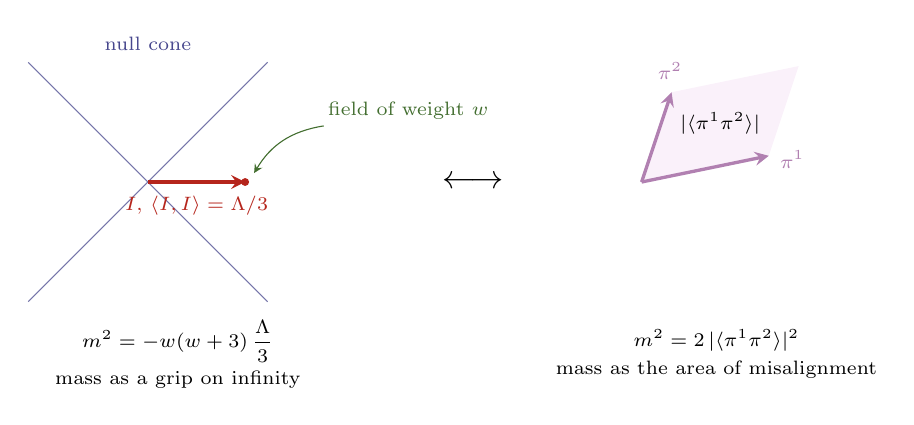
\begin{tikzpicture}[scale=0.95, >=stealth]
\begin{scope}
  \draw[MidnightBlue!60] (-1.6,-1.6) -- (1.6,1.6);
  \draw[MidnightBlue!60] (-1.6,1.6) -- (1.6,-1.6);
  \node[MidnightBlue!80, font=\scriptsize] at (0,1.85) {null cone};
  \draw[very thick, ->, BrickRed] (0,0) -- (1.3,0);
  \fill[BrickRed] (1.3,0) circle (1.5pt);
  \node[BrickRed, font=\scriptsize, below] at (0.65,-0.05) {$I$, $\ip{I}{I} = \Lambda/3$};
  \draw[OliveGreen!80!black, ->] (2.35,0.75) to[bend right=25] (1.42,0.12);
  \node[OliveGreen!80!black, font=\scriptsize, anchor=west] at (2.28,0.95) {field of weight $w$};
  \node[font=\scriptsize, align=center] at (0.4,-2.3)
    {$m^{2} = -w(w+3)\,\dfrac{\Lambda}{3}$\\[2pt] mass as a grip on infinity};
\end{scope}
\node[font=\large] at (4.35,0) {$\longleftrightarrow$};
\begin{scope}[xshift=6.6cm]
  \fill[Plum!15] (0,0) -- (1.7,0.35) -- (2.1,1.55) -- (0.4,1.2) -- cycle;
  \draw[very thick, ->, Plum!80!black] (0,0) -- (1.7,0.35);
  \draw[very thick, ->, Plum!80!black] (0,0) -- (0.4,1.2);
  \node[Plum!80!black, font=\scriptsize, anchor=west] at (1.72,0.3) {$\pi^{1}$};
  \node[Plum!80!black, font=\scriptsize, anchor=south] at (0.38,1.24) {$\pi^{2}$};
  \node[font=\scriptsize] at (1.05,0.78) {$|\br{\pi^{1}\pi^{2}}|$};
  \node[font=\scriptsize, align=center] at (1.0,-2.3)
    {$m^{2} = 2\,|\br{\pi^{1}\pi^{2}}|^{2}$\\[2pt] mass as the area of misalignment};
\end{scope}
\end{tikzpicture}
\caption{One grip, two readings. Left: the dictionary of Theorem \ref{thm:dictionary}: a field's mass is its conformal weight read against the frozen point's length, the one scale the theory contains. Right: the area formula of Proposition \ref{prop:area}: a composite's mass is the symplectic area by which its constituents' spinor parts fail to align; aligned constituents give a null composite. The link is Theorem \ref{thm:grip}: at $\Lambda = 0$ the bracket is the pairing of the composite against the frozen point, $m^{2} = 2|\ip{I}{Z^{1}\wedge Z^{2}}|^{2}$, and for $\Lambda \neq 0$ the composite's grip on the frozen point has squared length $2|B_{\Lambda}|^{2} + (\Lambda/3)\,C$. Both panels read the same object, the frozen point; the dictionary then assigns a composite heavier than $3H/2$ the weight $w = -\tfrac32 \pm i\nu$ with $\nu \approx m/H$ (Proposition \ref{prop:weight}).}
\label{fig:twolanguages}
\end{figure}

\begin{remark}[Point of contact: the angle between two vacua]\label{rem:vacua}
The twistor paper proves that a twistor is a state of the completion's three ladder pairs, a pure spinor, and that each twistor determines a Fock vacuum \cite[Thm.~5.3]{ButlerT9}. Under that identification the bracket $\br{\pi^{1}\pi^{2}}$ is the overlap datum of the two constituents' vacua, and Proposition \ref{prop:area} acquires its structural reading: a composite is massless exactly when its constituents agree on a vacuum, and mass is the area of their disagreement. Mass, in this reading, is not a quantity intrinsic to one constituent but a relation: a misalignment within the composite, on the twistor side; a grip on infinity, on the tractor side. That these are the same number is the join of the next section. The two-twistor description of massive particles is classical \cite{PenroseRindler1986, Hughston1979}; what the series adds is the identification of the ambient objects on both sides of the pairing, which is what lets the join be computed rather than postulated.
\end{remark}

\section{The exact join}\label{sec:join}

Theorem \ref{thm:dictionary} and Proposition \ref{prop:area} both compute a mass. This section shows that the flat-space formula is the squared pairing of the composite against the frozen point, extends it to $\Lambda \neq 0$ exactly, and then reads the composite's weight off the dictionary. The plan: find the frozen point of de Sitter space in the flat chart and fix what the chart's normalisation does and does not decide (Lemma \ref{lem:dsscale}, Remark \ref{rem:nullity}); write the conformal generators in the chart (Lemma \ref{lem:chartiso}); define the grip of a composite on the frozen point, which is its de Sitter momentum, and prove it is a real vector (Definition \ref{def:grip}, Lemma \ref{lem:real}); compute its squared length in closed form (Theorem \ref{thm:grip}); recognise the result as a difference of Casimirs (Proposition \ref{prop:casimir}) and identify the five broken generators (Lemma \ref{lem:five}); and read off the composite's weight (Proposition \ref{prop:weight}).

\subsection{The de Sitter scale in the flat chart}

\begin{lemma}[The de Sitter scale and its frozen point]\label{lem:dsscale}
Let $\eta$ be the flat metric on the chart of Fact \ref{fact:chart}, $Q(x) = \eta(x,x)$, and $\sigma(x) := 1 - \Lambda Q(x)/12$.
\begin{enumerate}
\item The scale tractor of $\sigma$ in the flat scale is
\[
I_{\sigma} = \bigl(\sigma,\; \nabla\sigma,\; -\tfrac14\Box\sigma\bigr) = \Bigl(1 - \frac{\Lambda Q}{12},\; -\frac{\Lambda}{6}\,x_{a},\; \frac{\Lambda}{6}\Bigr),
\]
it is parallel for the connection \eqref{eq:tractorconn} of $\eta$, and $\ip{I_{\sigma}}{I_{\sigma}} = \Lambda/3$ identically. Hence $g = \sigma^{-2}\eta$ is Einstein with cosmological constant $\Lambda$, on the region $\sigma \neq 0$: it is de Sitter space in the flat conformal chart, and $I_{\sigma}$ is its frozen point.
\item The constant ambient vector whose scale function is $\sigma$ is
\[
I_{\Lambda} := n_{\infty} + \frac{\Lambda}{6}\, n_{0},
\]
and it is the only one: $\ip{X(x)}{n_{\infty} + \lambda n_{0}} = 1 - \lambda Q(x)/2$, which equals $\sigma$ iff $\lambda = \Lambda/6$, and the points $X(x)$ span the ambient space. The vector $n_{0} + \lambda n_{\infty}$, of the same norm, has scale function $\lambda - Q/2$: the inverted chart, not this one.
\item $\ip{I_{\Lambda}}{I_{\Lambda}} = 2 \cdot \tfrac{\Lambda}{6}\ip{n_{\infty}}{n_{0}} = \Lambda/3$, in agreement with (1). At $\Lambda = 0$, $I_{\Lambda} = n_{\infty}$: the frozen point of flat space is the infinity twistor, and it becomes non-simple exactly when $\Lambda \neq 0$.
\end{enumerate}
\end{lemma}

\begin{proof}
\emph{(1) The scale tractor.} By Fact \ref{fact:thomas} at $w = 1$ with $J = 0$ for the flat scale, the scale tractor of $\sigma$ is $\tfrac14 D\sigma = (\sigma, \nabla\sigma, -\tfrac14\Box\sigma)$. With $\nabla_{a}Q = 2x_{a}$ and $\Box Q = 2\eta^{ab}\eta_{ab} = 8$,
\[
\nabla_{a}\sigma = -\tfrac{\Lambda}{6}\,x_{a}, \qquad \Box\sigma = -\tfrac{2\Lambda}{3}, \qquad -\tfrac14\Box\sigma = \tfrac{\Lambda}{6}.
\]
\emph{Parallelism}, slot by slot in \eqref{eq:tractorconn} with $P = 0$: the first slot is $\nabla_{a}\sigma - \mu_{a} = 0$ by construction; the second is $\nabla_{a}\mu_{b} + \eta_{ab}\rho = -\tfrac{\Lambda}{6}\eta_{ab} + \tfrac{\Lambda}{6}\eta_{ab} = 0$; the third is $\nabla_{a}\rho = 0$ since $\rho$ is constant. \emph{The norm:}
\[
2\sigma\rho + \eta^{ab}\mu_{a}\mu_{b} = 2\Bigl(1 - \frac{\Lambda Q}{12}\Bigr)\frac{\Lambda}{6} + \frac{\Lambda^{2}}{36}Q = \frac{\Lambda}{3}.
\]
\emph{Einstein.} The tractor metric and parallelism are scale-independent, so in the scale $\sigma$ itself, where the density is the constant $1$ and the section therefore reads $(1, 0, \rho')$ by Fact \ref{fact:thomas} (its middle slot is $n\nabla 1 = 0$), with $2\rho' = \Lambda/3$, Fact \ref{fact:frozen} gives that $g = \sigma^{-2}\eta$ is Einstein with $P_{ab} = \rho' g_{ab}$, that is with cosmological constant $6\rho' = \Lambda$.

\emph{(2) The flat-model dictionary.} In the form used here it is elementary. A section $(\sigma, \mu_{b}, \rho)$ is parallel for \eqref{eq:tractorconn} with $P = 0$ iff the three slot equations $\nabla_{a}\rho = 0$, $\nabla_{a}\mu_{b} = -\eta_{ab}\rho$, $\nabla_{a}\sigma = \mu_{a}$ hold; integrating them in turn,
\[
\rho = \text{const}, \qquad \mu_{b} = v_{b} - \rho\, x_{b}, \qquad \sigma = \alpha + \ip{v}{x} - \tfrac12\rho\, Q(x),
\]
with $v$ a constant covector and $\alpha$ a constant: a six-parameter family. Since $\ip{X(x)}{\alpha n_{\infty} + \rho n_{0} + v} = \alpha - \tfrac12\rho Q(x) + \ip{v}{x}$ is exactly this $\sigma$-slot, the parallel sections are the constant vectors $V = \alpha n_{\infty} + \rho n_{0} + v$, with scale function $\ip{X(x)}{V}$.

\emph{The scale function of $I_{\Lambda}$.} $\ip{X(x)}{n_{\infty}} = \ip{n_{0}}{n_{\infty}} = 1$ and $\ip{X(x)}{n_{0}} = -\tfrac12 Q\ip{n_{\infty}}{n_{0}} = -\tfrac12 Q$, since $n_{0}, n_{\infty}$ are null and orthogonal to $x$; so
\[
\ip{X(x)}{n_{\infty} + \lambda n_{0}} = 1 - \tfrac12\lambda Q(x), \qquad \ip{X(x)}{n_{0} + \lambda n_{\infty}} = \lambda - \tfrac12 Q(x),
\]
and the first equals $\sigma$ iff $\lambda = \Lambda/6$.

\emph{Uniqueness.} The scale function $x \mapsto \ip{X(x)}{V}$ determines $V$ because the vectors $X(x)$ span the ambient space: the six values at $x = 0$, at the four coordinate unit vectors $e_{a}$ of $\eta$, and at $x = 2e_{0}$ are independent, since $X(0) = n_{0}$, $X(e_{a}) - X(0) = e_{a} - \tfrac12\eta_{aa}n_{\infty}$, and $X(2e_{0}) - 2X(e_{0}) + X(0) = -n_{\infty}$.

\emph{(3) The norm in the chart.} $\ip{n_{\infty} + \lambda n_{0}}{n_{\infty} + \lambda n_{0}} = 2\lambda\ip{n_{\infty}}{n_{0}} = 2\lambda$, using $\ip{n_{\infty}}{n_{\infty}} = \ip{n_{0}}{n_{0}} = 0$; and by Fact \ref{fact:chart} a bivector is simple iff its norm vanishes, so $n_{\infty} + \lambda n_{0}$ is simple iff $\lambda = 0$. The general statement behind (3), that the infinity twistor is simple iff $\Lambda = 0$, is \cite[Cor.~4.8]{ButlerT9}; here it is the chart computation.

\emph{Script.} It confirms (1) as rational-function identities in $\Lambda$ at rational points (the second slot of the connection, the only one that is not an identity by construction, and the norm $\Lambda/3$), the scale-function values of (2) at rational points and three values of $\lambda$ together with the spanning of the six listed points by exact rank, and the ambient norm of (3) formed and equal to $2\lambda$ at four values (null, hence simple by Fact \ref{fact:chart}, exactly at $\lambda = 0$).
\end{proof}

\begin{remark}[What nullity fixes]\label{rem:nullity}
With the undetermined slot coefficient $X_{c}(x) = n_{0} + x + c\,Q(x)\,n_{\infty}$ one has $\ip{X_{c}}{X_{c}} = Q(x)(1 + 2c)$, so nullity of the point embedding for all $x$ fixes $c = -\tfrac12$. This is a statement about the coefficient, not about the chart's normalisation: rescaling the volume form $\varepsilon$ by $\kappa$ rescales $\ip{n_{0}}{n_{\infty}}$, $\ip{x}{x}$ and $\ip{X_{c}}{X_{c}}$ alike, and nullity is insensitive to $\kappa$. What fixes the chart is the imported normalisation $\ip{n_{0}}{n_{\infty}} = +1$ together with $Q = \ip{x}{x}$ (Fact \ref{fact:chart}); on the $x$-slot this reads $\ip{x}{y} = -\varepsilon_{ab}\varepsilon_{a'b'}x^{aa'}y^{bb'}$, so $Q(x) = -2\det(x^{aa'})$. The real points of the $x$-slot are, by definition, the $x$ whose translation generator $A(x\wedge n_{\infty})$ lies in $\mathfrak{su}(2,2)$ for the Hermitian form \eqref{eq:hermitian} fixed below; by Lemma \ref{lem:chartiso}(2) that generator's block is $b_{x} = x\varepsilon$, and $x\varepsilon$ is anti-Hermitian iff $x = \tfrac{i}{\sqrt2}K\varepsilon$ with $K$ Hermitian (if $x = \tfrac{i}{\sqrt2}K\varepsilon$ then $x\varepsilon = -\tfrac{i}{\sqrt2}K$; conversely $K := i\sqrt2\,x\varepsilon$ is Hermitian when $x\varepsilon$ is anti-Hermitian, and $x = -\tfrac{i}{\sqrt2}K\varepsilon^{-1} = \tfrac{i}{\sqrt2}K\varepsilon$). So the real points are the matrices
\begin{equation}\label{eq:realslice}
x^{aa'} = \frac{i}{\sqrt2}\,K\varepsilon, \qquad K = \begin{pmatrix} x^{0}+x^{3} & x^{1}-ix^{2} \\ x^{1}+ix^{2} & x^{0}-x^{3}\end{pmatrix},\quad \varepsilon = \begin{pmatrix} 0 & 1 \\ -1 & 0\end{pmatrix},
\end{equation}
with $(x^{0}, x^{1}, x^{2}, x^{3})$ real, on which $Q = -2\det x = \det K = (x^{0})^{2} - (x^{1})^{2} - (x^{2})^{2} - (x^{3})^{2}$; the factor $i$ is that of the incidence relation, and the factor $\varepsilon$ is what makes the translation generators of Lemma \ref{lem:chartiso} anti-Hermitian for \eqref{eq:hermitian} (Lemma \ref{lem:real}). The twistor paper's reality structure \cite[Prop.~4.5]{ButlerT9} selects the same slice up to a choice of frame in $\Sc'$, which changes no formula of this section: the computations below are polynomial identities in the chart. The script checks these statements with the slice scaled by $\sqrt2$ (so that $Q = 2\det K$ there), the normalisation $1/\sqrt2$ being a real scalar that affects no reality statement; it also confirms that the anti-Hermiticity condition on the eight real parameters of $x$ has rank four, so that the slice is all of the real locus.
\end{remark}

\subsection{The conformal generators in the chart}

Write $\T = \Sc \oplus \Sc'$ with bases $e_{1}, e_{2}$ of $\Sc$ and $e_{3}, e_{4}$ of $\Sc'$, so that $n_{\infty} = e_{1}\wedge e_{2}$, $n_{0} = e_{3}\wedge e_{4}$, the $x$-slot is spanned by the mixed bivectors $e_{a}\wedge e_{a'}$ ($a \in \{1,2\}$, $a' \in \{3,4\}$), and $\varepsilon(e_{1}\wedge e_{2}\wedge e_{3}\wedge e_{4}) = 1$, which gives $\ip{n_{0}}{n_{\infty}} = +1$. A twistor is $Z = \omega + \pi = \omega^{a}e_{a} + \pi^{a'}e_{a'}$. Let $\varepsilon_{ab}$ and $\varepsilon_{a'b'}$ be the antisymmetric symbols with $\varepsilon_{12} = \varepsilon_{34} = 1$, so that $e_{a}\wedge e_{b} = \varepsilon_{ab}\,n_{\infty}$, $e_{a'}\wedge e_{b'} = \varepsilon_{a'b'}\,n_{0}$, and the brackets are the determinants $\br{\pi^{1}\pi^{2}} := \varepsilon_{a'b'}\pi_{1}^{a'}\pi_{2}^{b'}$ and $[\omega^{1}\omega^{2}] := \varepsilon_{ab}\omega_{1}^{a}\omega_{2}^{b}$. For the ambient vector $U \wedge V$ let $R_{U\wedge V}$ be the rotation $W \mapsto \ip{U}{W}V - \ip{V}{W}U$ of $\Lambda^{2}\T$, and let $A(U \wedge V) \in \mathfrak{sl}(\T)$ be its preimage under the isomorphism of Fact \ref{fact:chart}. Matrices act on column vectors in the basis $(e_{1}, e_{2}, e_{3}, e_{4})$, in block form according to $\Sc \oplus \Sc'$.

\begin{lemma}[The chart form of the spin isomorphism]\label{lem:chartiso}
For $x = x^{aa'}e_{a}\wedge e_{a'}$ in the $x$-slot:
\begin{enumerate}
\item $A(n_{\infty}\wedge n_{0}) = \operatorname{diag}(-\tfrac12, -\tfrac12, \tfrac12, \tfrac12)$, the grading element;
\item $A(x \wedge n_{\infty}) = \begin{pmatrix} 0 & b_{x} \\ 0 & 0 \end{pmatrix}$ with $b_{x}: \Sc' \to \Sc$, $(b_{x}\pi)^{a} = x^{aa'}\varepsilon_{a'b'}\pi^{b'}$: the translations;
\item $A(x \wedge n_{0}) = \begin{pmatrix} 0 & 0 \\ c_{x} & 0 \end{pmatrix}$ with $c_{x}: \Sc \to \Sc'$, $(c_{x}\omega)^{a'} = -x^{ba'}\varepsilon_{ba}\omega^{a}$: the special conformal generators.
\end{enumerate}
\end{lemma}

\begin{proof}
Since the map $A \mapsto (U \mapsto A\cdot U)$ is an isomorphism onto $\mathfrak{so}(\Lambda^{2}\T,\varepsilon)$, it suffices to check that each displayed matrix acts on the six basis bivectors as the named rotation does. Throughout, $\ip{n_{\infty}}{n_{\infty}} = \ip{n_{0}}{n_{0}} = 0$, $\ip{n_{\infty}}{n_{0}} = 1$, and the $x$-slot is orthogonal to both.

(1) $R_{n_{\infty}\wedge n_{0}}$ sends $n_{\infty} \mapsto \ip{n_{\infty}}{n_{\infty}}n_{0} - \ip{n_{0}}{n_{\infty}}n_{\infty} = -n_{\infty}$, $n_{0} \mapsto n_{0}$, and every $x$-slot vector to $0$. The matrix $\operatorname{diag}(-\tfrac12,-\tfrac12,\tfrac12,\tfrac12)$ sends $e_{1}\wedge e_{2} \mapsto (-\tfrac12 - \tfrac12)e_{1}\wedge e_{2} = -n_{\infty}$, $e_{3}\wedge e_{4} \mapsto n_{0}$, and $e_{a}\wedge e_{a'} \mapsto (-\tfrac12 + \tfrac12)e_{a}\wedge e_{a'} = 0$.

(2) $R_{x\wedge n_{\infty}}$ sends $n_{\infty} \mapsto \ip{x}{n_{\infty}}n_{\infty} - \ip{n_{\infty}}{n_{\infty}}x = 0$, a mixed bivector $y \mapsto \ip{x}{y}n_{\infty}$, and $n_{0} \mapsto \ip{x}{n_{0}}n_{\infty} - \ip{n_{\infty}}{n_{0}}x = -x$. The matrix $A$ with block $b_{x}$ annihilates $\Sc$ and maps $e_{b'} \mapsto x^{aa'}\varepsilon_{a'b'}e_{a}$. Hence $A\cdot n_{\infty} = Ae_{1}\wedge e_{2} + e_{1}\wedge Ae_{2} = 0$. For $y = e_{c}\wedge e_{b'}$: $A\cdot y = e_{c}\wedge Ae_{b'} = x^{aa'}\varepsilon_{a'b'}\,e_{c}\wedge e_{a} = x^{aa'}\varepsilon_{a'b'}\varepsilon_{ca}\,n_{\infty}$, while by Remark \ref{rem:nullity} $\ip{x}{e_{c}\wedge e_{b'}} = -\varepsilon_{ac}\varepsilon_{a'b'}x^{aa'} = \varepsilon_{ca}\varepsilon_{a'b'}x^{aa'}$: equal. For $n_{0}$: $A\cdot(e_{3}\wedge e_{4}) = Ae_{3}\wedge e_{4} + e_{3}\wedge Ae_{4} = x^{a4}\varepsilon_{43}\,e_{a}\wedge e_{4} + x^{a3}\varepsilon_{34}\,e_{3}\wedge e_{a} = -x^{a4}e_{a}\wedge e_{4} - x^{a3}e_{a}\wedge e_{3} = -x$.

(3) $R_{x\wedge n_{0}}$ sends $n_{0} \mapsto 0$, $y \mapsto \ip{x}{y}n_{0}$, and $n_{\infty} \mapsto \ip{x}{n_{\infty}}n_{0} - \ip{n_{0}}{n_{\infty}}x = -x$. The matrix with block $c_{x}$ annihilates $\Sc'$ and maps $e_{a} \mapsto -x^{ba'}\varepsilon_{ba}e_{a'}$. Hence $A\cdot n_{0} = 0$. For $y = e_{a}\wedge e_{c'}$: $A\cdot y = Ae_{a}\wedge e_{c'} = -x^{ba'}\varepsilon_{ba}\,e_{a'}\wedge e_{c'} = -x^{ba'}\varepsilon_{ba}\varepsilon_{a'c'}\,n_{0}$, while $\ip{x}{e_{a}\wedge e_{c'}} = -\varepsilon_{ba}\varepsilon_{a'c'}x^{ba'}$: equal. For $n_{\infty}$: $A\cdot(e_{1}\wedge e_{2}) = Ae_{1}\wedge e_{2} + e_{1}\wedge Ae_{2} = -x^{2a'}\varepsilon_{21}\,e_{a'}\wedge e_{2} - x^{1a'}\varepsilon_{12}\,e_{1}\wedge e_{a'} = -x^{2a'}e_{2}\wedge e_{a'} - x^{1a'}e_{1}\wedge e_{a'} = -x$.

Each displayed matrix is traceless. The script solves the linear systems $A\cdot P = R(P)$ exactly for the nine rotations displayed and confirms that the solutions are these matrices, entry by entry.
\end{proof}

\subsection{The grip of a composite on the frozen point}

The classical phase space of $N$ twistors carries the Hermitian form $\Sigma$ of signature $(2,2)$, written $\bar{Z}\cdot W := \Sigma(Z, W)$, and the conformal group acts by $SU(2,2)$. The form is canonical up to a phase and has signature $(2,2)$ \cite[Prop.~4.5(1), (2), (4)]{ButlerT9}; the chart frame fixes the phase, and in it $\Sigma$ is the standard twistor form $\bar{Z}\cdot Z = \omega^{A}\bar\pi_{A} + \bar\omega^{A'}\pi_{A'}$ \cite{PenroseRindler1986}, which pairs $\omega$ with $\bar\pi$ through the frame: for $Z = (\omega, \pi)$ and $W = (\xi, \chi)$,
\begin{equation}\label{eq:hermitian}
\bar{Z}\cdot W = \hp{\pi}{\xi} + \overline{\hp{\chi}{\omega}}, \qquad \hp{u}{v} := \overline{u^{3}}\,v^{1} + \overline{u^{4}}\,v^{2}\quad (u \in \Sc',\ v \in \Sc),
\end{equation}
the sesquilinear pairing that identifies the frame $e_{3}, e_{4}$ of $\Sc'$ with the frame $e_{1}, e_{2}$ of $\Sc$; we write $\bar{u}_{a}$ for the conjugate of the component of $u \in \Sc'$ so identified with $e_{a}$, so that $\hp{u}{v} = \bar{u}_{a}v^{a}$. The real slice \eqref{eq:realslice} is the one this form determines. The moment map of the action on the phase space is the classical form of the generators of Fact \ref{fact:chart}:
\begin{equation}\label{eq:moment}
M_{A}(Z^{1}, \dots, Z^{N}) := i\sum_{i=1}^{N} \bar{Z}^{i}\cdot(A Z^{i}), \qquad A \in \mathfrak{sl}(\T),
\end{equation}
real for $A \in \mathfrak{su}(2,2)$, and $M_{U\wedge V} := M_{A(U\wedge V)}$ for ambient $U, V$. Equivariance is built in: for $\gamma \in SU(2,2)$, $M_{A}(\gamma Z) = M_{\gamma^{-1}A\gamma}(Z)$, and $A(\gamma U \wedge \gamma V) = \gamma\,A(U\wedge V)\,\gamma^{-1}$ because the isomorphism of Fact \ref{fact:chart} intertwines the two actions.

\begin{definition}[The grip, and the mass of a composite]\label{def:grip}
Let $I$ be a nonzero ambient vector and $Z^{1}, \dots, Z^{N}$ a composite. The \emph{grip} of the composite on $I$ is the ambient vector $P = M(I)$ determined by
\[
\ip{P}{U} = M_{U\wedge I} \qquad\text{for all ambient } U,
\]
which exists and is unique because the pairing is nondegenerate. The \emph{mass-squared} of the composite relative to $I$ is $m^{2} := \ip{P}{P}$.
\end{definition}

Three properties follow at once. First, $\ip{P}{I} = M_{I\wedge I} = 0$: the grip lies in $I^{\perp}$. Second, $m^{2}$ is invariant under the stabiliser of $I$: for $\gamma$ with $\gamma I = I$, $\ip{P(\gamma Z)}{U} = M_{U\wedge I}(\gamma Z) = M_{\gamma^{-1}(U\wedge I)}(Z) = M_{\gamma^{-1}U\wedge I}(Z) = \ip{P(Z)}{\gamma^{-1}U} = \ip{\gamma P(Z)}{U}$, so $P(\gamma Z) = \gamma P(Z)$ and $\ip{P}{P}$ is unchanged; for the frozen point of Lemma \ref{lem:dsscale} the stabiliser acts on the ambient space through $SO(1,4)$ (Fact \ref{fact:frozen}; the Lie-algebra form of the surjection is Lemma \ref{lem:five}), and $P$ is a de Sitter vector. Third, at $\Lambda = 0$, $I = n_{\infty}$ and $\ip{P}{x} = M_{x\wedge n_{\infty}}$ is, by Lemma \ref{lem:chartiso}(2), the value of the translation generator on the composite, that is, its total momentum in the direction $x$; the $x$-slot part of $P$ is therefore the momentum, the remaining part is $-d\,n_{\infty}$ with $d$ the dilation charge, and since $n_{\infty}$ is null and orthogonal to the $x$-slot, $m^{2}$ is the Poincar\'e Casimir $p^{2}$. Definition \ref{def:grip} is the de Sitter extension of the mass of Proposition \ref{prop:area}: the composite's momentum is its grip on the point at infinity, and its mass is the length of that grip. Lemma \ref{lem:five} below identifies the generators $A(e_{a}\wedge I)$, $e_{a} \in I^{\perp}$, whose charges are the components of $P$, with the five generators of $\mathfrak{su}(2,2)$ broken by $I$, the de Sitter translations, which is the representation-theoretic form of the same statement. That $P$ is a real vector, so that $\ip{P}{P}$ is a value of the real $(1,4)$ form on $I^{\perp}$, is the next lemma.

\begin{lemma}[The grip is real]\label{lem:real}
Let $V_{\R}$ be the real span of $n_{\infty}$, $n_{0}$ and the real slice \eqref{eq:realslice} of the $x$-slot. For $U, V \in V_{\R}$ the generator $A(U\wedge V)$ lies in $\mathfrak{su}(2,2)$, the real form of $\Sigma$; hence $M_{U\wedge V}$ is real, and for $I \in V_{\R}$ the grip $P = M(I)$ lies in $V_{\R}$. For the frozen point $I_{\Lambda}$, $P$ is a real vector of $I_{\Lambda}^{\perp}$ and $m^{2} = \ip{P}{P}$ is a value of the $(1,4)$ form of Fact \ref{fact:frozen}.
\end{lemma}

\begin{proof}
The first conclusion is the chart form of \cite[Prop.~4.5(2)]{ButlerT9}, which states that the real bivectors act $\Sigma$-anti-Hermitianly; here it is the chart computation, in four steps. The second conclusion is this paper's.

\emph{Step 1, the criterion.} In the block form of Lemma \ref{lem:chartiso}, $\Sigma = \left(\begin{smallmatrix} 0 & 1 \\ 1 & 0\end{smallmatrix}\right)$, so for $A = \left(\begin{smallmatrix} A_{11} & A_{12} \\ A_{21} & A_{22}\end{smallmatrix}\right)$ the matrix $\Sigma A = \left(\begin{smallmatrix} A_{21} & A_{22} \\ A_{11} & A_{12}\end{smallmatrix}\right)$ is anti-Hermitian iff $A_{12}^{\dagger} = -A_{12}$, $A_{21}^{\dagger} = -A_{21}$ and $A_{22} = -A_{11}^{\dagger}$.

\emph{Step 2, the grading and the translations.} The grading element has $A_{11} = -\tfrac12$, $A_{22} = \tfrac12$, $A_{12} = A_{21} = 0$, and satisfies the criterion. For $x$ in the slice \eqref{eq:realslice}, $x = \tfrac{i}{\sqrt2}K\varepsilon$ with $K$ Hermitian, the translation block of Lemma \ref{lem:chartiso}(2) is $b_{x} = x\varepsilon = \tfrac{i}{\sqrt2}K\varepsilon^{2} = -\tfrac{i}{\sqrt2}K$, anti-Hermitian.

\emph{Step 3, the special conformal generators.} The block of Lemma \ref{lem:chartiso}(3) is $c_{x} = -x^{\mathsf T}\varepsilon = \tfrac{i}{\sqrt2}\,\varepsilon K^{\mathsf T}\varepsilon$ (using $\varepsilon^{\mathsf T} = -\varepsilon$), whose adjoint is $-\tfrac{i}{\sqrt2}\,\varepsilon^{\dagger}\bar{K}\varepsilon^{\dagger} = -\tfrac{i}{\sqrt2}\,\varepsilon K^{\mathsf T}\varepsilon = -c_{x}$, since $\bar K = K^{\mathsf T}$ and $\varepsilon^{\dagger} = -\varepsilon$: anti-Hermitian.

\emph{Step 4, the Lorentz generators.} For two rotations $R_{U\wedge V}(Z) = \ip{U}{Z}V - \ip{V}{Z}U$, expanding both sides on a vector $Z$ gives
\[
[R_{U\wedge V}, R_{W\wedge Y}] = \ip{U}{W}R_{V\wedge Y} - \ip{U}{Y}R_{V\wedge W} - \ip{V}{W}R_{U\wedge Y} + \ip{V}{Y}R_{U\wedge W}
\]
(the four terms are $R_{U\wedge V}R_{W\wedge Y}Z = \ip{W}{Z}\,R_{U\wedge V}Y - \ip{Y}{Z}\,R_{U\wedge V}W$ minus the same with the pairs exchanged, regrouped by which of $U, V, W, Y$ carries $Z$). For $U = x$, $V = n_{\infty}$, $W = x'$, $Y = n_{0}$ with $x, x'$ in the slice, $\ip{n_{\infty}}{x'} = \ip{x}{n_{0}} = \ip{n_{\infty}}{n_{\infty}} = 0$ and $\ip{n_{\infty}}{n_{0}} = 1$ leave $[R_{x\wedge n_{\infty}}, R_{x'\wedge n_{0}}] = \ip{x}{x'}R_{n_{\infty}\wedge n_{0}} + R_{x\wedge x'}$. Hence $A(x\wedge x') = [A(x\wedge n_{\infty}), A(x'\wedge n_{0})] - \ip{x}{x'}A(n_{\infty}\wedge n_{0})$ lies in $\mathfrak{su}(2,2)$, a Lie algebra, because $\ip{x}{x'}$ is real.

\emph{The span, and the grip.} The pairs $n_{\infty}\wedge n_{0}$ (one), $x\wedge n_{\infty}$ (four), $x\wedge n_{0}$ (four) and $x\wedge x'$ (six) span $\Lambda^{2}V_{\R}$, of dimension $15$, so every $A(U\wedge V)$ with $U, V \in V_{\R}$ is in $\mathfrak{su}(2,2)$, and $M_{A}$ is real there because $\Sigma A$ anti-Hermitian makes $\bar{Z}\cdot AZ$ imaginary. Then $\ip{P}{U} = M_{U\wedge I}$ is real for every $U \in V_{\R}$, and since the pairing restricted to $V_{\R}$ is a real nondegenerate form (the form of signature $(2,4)$ of Fact \ref{fact:chart}; in the basis $n_{\infty}, n_{0}$ and the slice \eqref{eq:realslice} its Gram matrix is $\left(\begin{smallmatrix} 0 & 1 \\ 1 & 0\end{smallmatrix}\right) \oplus \operatorname{diag}(1,-1,-1,-1)$), $P \in V_{\R}$. The last clause is $P \perp I_{\Lambda}$ with Fact \ref{fact:frozen}. The script checks the commutator identity on the real points, the anti-Hermiticity of the generators for real pairs on four real points, and the reality of the pairings of $P$ with a real basis of $V_{\R}$.
\end{proof}

For two twistors, write $t_{il} := \hp{\pi^{i}}{\omega^{l}}$ ($i, l \in \{1,2\}$) for the $2 \times 2$ matrix of mixed pairings, and
\begin{equation}\label{eq:gram}
h_{il} := \bar{Z}^{i}\cdot Z^{l} = t_{il} + \overline{t_{li}}, \qquad
C := \tfrac14\,(h_{11} - h_{22})^{2} + |h_{12}|^{2} = \tfrac12\tr\bigl(h_{0}^{2}\bigr) = \tfrac14\bigl[(\tr h)^{2} - 4\det h\bigr],
\end{equation}
for the Hermitian Gram matrix $h$ of the composite and its traceless part $h_{0}$. The diagonal entries $h_{ii} = \bar{Z}^{i}\cdot Z^{i}$ are twice the constituents' helicities; $C$ is the quadratic Casimir of the internal $\mathfrak{su}(2)$ that mixes the two constituents, a quarter of the squared difference of the eigenvalues of $h$, nonnegative, and zero exactly when $h$ is a multiple of the identity.

\begin{theorem}[The exact join]\label{thm:grip}
Let $I_{\Lambda} = n_{\infty} + \lambda n_{0}$ with $\lambda = \Lambda/6$ be the frozen point of Lemma \ref{lem:dsscale}, and $Z^{1}, Z^{2}$ two twistors.
\begin{enumerate}
\item \emph{(The deformed bracket.)} The pairing of the composite against the frozen point is
\begin{equation}\label{eq:blambda}
B_{\Lambda} := \ip{I_{\Lambda}}{Z^{1}\wedge Z^{2}} = \br{\pi^{1}\pi^{2}} + \frac{\Lambda}{6}\,[\omega^{1}\omega^{2}],
\end{equation}
and at $\Lambda = 0$ it is the classical contraction of the composite with the infinity twistor.
\item \emph{(The mass.)} The grip $P = M(I_{\Lambda})$ has squared length
\begin{equation}\label{eq:grip}
m^{2} = \ip{P}{P} = 2\,|B_{\Lambda}|^{2} + \ip{I_{\Lambda}}{I_{\Lambda}}\, C = 2\,|B_{\Lambda}|^{2} + \frac{\Lambda}{3}\, C .
\end{equation}
\item \emph{(The flat shadow.)} At $\Lambda = 0$, $m^{2} = 2|\ip{I}{Z^{1}\wedge Z^{2}}|^{2} = 2|\br{\pi^{1}\pi^{2}}|^{2}$: Proposition \ref{prop:area}, read as the squared pairing of the composite against the frozen point.
\item \emph{(The point-supported composite.)} If both twistors lie on the incidence line of the point $x$, the composite bivector is $\br{\pi^{1}\pi^{2}}X(x)$ and $B_{\Lambda} = \sigma(x)\br{\pi^{1}\pi^{2}} = \bigl(1 - \tfrac{\Lambda Q(x)}{12}\bigr)\br{\pi^{1}\pi^{2}}$: the flat bracket read in the de Sitter scale.
\item \emph{(The massless locus.)} For $\Lambda > 0$, $m^{2} \ge 0$, and $m^{2} = 0$ if and only if $B_{\Lambda} = 0$ and $h$ is a multiple of the identity. The doubled composite $Z^{2} = Z^{1}$ has $B_{\Lambda} = 0$ and $m^{2} = \tfrac{\Lambda}{3}\,(\bar{Z}\cdot Z)^{2}$, so it is massless only when its constituent is null; and there are massless composites that are not doubled, for instance $Z^{1} = e_{1} + e_{4}$, $Z^{2} = \alpha e_{1} + \beta e_{4}$ with $\alpha \neq \beta$.
\end{enumerate}
\end{theorem}

\begin{proof}
(1) Expand $Z^{1}\wedge Z^{2} = (\omega^{1} + \pi^{1})\wedge(\omega^{2} + \pi^{2})$ into four terms. Pairing against $n_{\infty} = e_{1}\wedge e_{2}$ annihilates every term with an $\omega$ factor (the wedge repeats a vector of $\Sc$), leaving $\varepsilon(e_{1}\wedge e_{2}\wedge\pi^{1}\wedge\pi^{2}) = \varepsilon_{a'b'}\pi_{1}^{a'}\pi_{2}^{b'}\,\varepsilon(e_{1}\wedge e_{2}\wedge e_{3}\wedge e_{4}) = \br{\pi^{1}\pi^{2}}$; pairing against $n_{0} = e_{3}\wedge e_{4}$ likewise leaves $\varepsilon(e_{3}\wedge e_{4}\wedge\omega^{1}\wedge\omega^{2}) = [\omega^{1}\omega^{2}]\,\varepsilon(e_{3}\wedge e_{4}\wedge e_{1}\wedge e_{2}) = [\omega^{1}\omega^{2}]$, the permutation being even. Linearity in $I_{\Lambda}$ gives \eqref{eq:blambda}; at $\Lambda = 0$ the infinity twistor is $n_{\infty}$ (Lemma \ref{lem:dsscale}(3)).

(2) \emph{Slots of the grip.} $M_{U\wedge I}$ is linear in $U \wedge I$, so with $I_{\Lambda} = n_{\infty} + \lambda n_{0}$ the grip is $P = P_{\infty} + \lambda P_{0}$, where $P_{\infty} := M(n_{\infty})$ and $P_{0} := M(n_{0})$. Put $d := M_{n_{\infty}\wedge n_{0}}$, and for $x$ in the $x$-slot $p(x) := M_{x\wedge n_{\infty}}$, $k(x) := M_{x\wedge n_{0}}$, three linear forms in $x$. Then $\ip{P}{n_{\infty}} = M_{n_{\infty}\wedge I_{\Lambda}} = \lambda M_{n_{\infty}\wedge n_{0}} = \lambda d$, $\ip{P}{n_{0}} = M_{n_{0}\wedge n_{\infty}} = -d$, and $\ip{P}{x} = p(x) + \lambda k(x)$. Writing $P = \alpha n_{\infty} + \beta n_{0} + v$ with $v$ in the $x$-slot, $\alpha = \ip{P}{n_{0}} = -d$, $\beta = \ip{P}{n_{\infty}} = \lambda d$, and $\ip{v}{x} = p(x) + \lambda k(x)$ for all $x$. Hence
\[
\ip{P}{P} = 2\alpha\beta + \ip{v}{v} = -2\lambda d^{2} + p\cdot p + 2\lambda\, p\cdot k + \lambda^{2}\, k\cdot k,
\]
where $f \cdot g$ denotes the dual metric on linear forms on the $x$-slot. By Remark \ref{rem:nullity} the metric matrix on the $x$-slot, in the components $x^{aa'}$, is $G = -\varepsilon\otimes\varepsilon$; since $\varepsilon^{2} = -1$, $G^{2} = (\varepsilon\otimes\varepsilon)^{2} = \varepsilon^{2}\otimes\varepsilon^{2} = 1$, so $G^{-1} = G$ and $f\cdot g = -\varepsilon_{ab}\varepsilon_{a'b'}f_{aa'}g_{bb'}$ with the same numerical symbols. Below, $u\cdot v$ for two $2$-component objects is the plain sum $\sum_{a}u_{a}v_{a}$ of products of components.

\emph{The three forms in components.} By Lemma \ref{lem:chartiso}(2), $A(x\wedge n_{\infty})Z = b_{x}\pi \in \Sc$, so by \eqref{eq:hermitian} and \eqref{eq:moment}, $p(x) = i\sum_{i}\hp{\pi^{i}}{b_{x}\pi^{i}} = i\sum_{i} x^{aa'}\,\overline{\pi^{i}_{a}}\,(\varepsilon\pi^{i})_{a'}$, where $(\varepsilon\pi)_{a'} := \varepsilon_{a'b'}\pi^{b'}$ and $\overline{\pi^{i}_{a}}$ is the conjugate of the component of $\pi^{i}$ paired with $e_{a}$ by $\Sigma$. Thus $p = \sum_{i}p^{i}$ with $p^{i}_{aa'} = i\,\overline{\pi^{i}_{a}}\,(\varepsilon\pi^{i})_{a'}$. By Lemma \ref{lem:chartiso}(3), $A(x\wedge n_{0})Z = c_{x}\omega \in \Sc'$, so $k(x) = i\sum_{i}\overline{\hp{c_{x}\omega^{i}}{\omega^{i}}} = i\sum_{i}\sum_{a'}(c_{x}\omega^{i})^{a'}\,\overline{\omega^{i}_{a'}} = -i\sum_{i}x^{ba'}\varepsilon_{ba}\omega^{i\,a}\,\overline{\omega^{i}_{a'}}$; thus $k = \sum_{i}k^{i}$ with $k^{i}_{aa'} = -i\,(\varepsilon\omega^{i})_{a}\,\overline{\omega^{i}_{a'}}$, where $(\varepsilon\omega)_{a} := \varepsilon_{ab}\omega^{b}$. By Lemma \ref{lem:chartiso}(1), $A(n_{\infty}\wedge n_{0})Z = (-\tfrac12\omega, \tfrac12\pi)$, so $\bar{Z}\cdot AZ = -\tfrac12\hp{\pi}{\omega} + \tfrac12\overline{\hp{\pi}{\omega}} = -i\,\mathrm{Im}\hp{\pi}{\omega}$ and $d = \sum_{i}\mathrm{Im}\,t_{ii} = \mathrm{Im}\tr t$.

\emph{The three pairings.} Using $\varepsilon^{\mathsf T}\varepsilon = 1$, $\varepsilon^{2} = -1$ and $\det\varepsilon = 1$ for the $2\times 2$ symbol:
\begin{align*}
p^{i}\cdot p^{l} &= -\varepsilon_{ab}\varepsilon_{a'b'}\,(i)^{2}\,\overline{\pi^{i}_{a}}\,\overline{\pi^{l}_{b}}\,(\varepsilon\pi^{i})_{a'}(\varepsilon\pi^{l})_{b'}
= \overline{\br{\pi^{i}\pi^{l}}}\;\br{\varepsilon\pi^{i},\varepsilon\pi^{l}} = |\br{\pi^{i}\pi^{l}}|^{2},\\
k^{i}\cdot k^{l} &= -\varepsilon_{ab}\varepsilon_{a'b'}\,(-i)^{2}\,(\varepsilon\omega^{i})_{a}(\varepsilon\omega^{l})_{b}\,\overline{\omega^{i}_{a'}}\,\overline{\omega^{l}_{b'}}
= [\varepsilon\omega^{i},\varepsilon\omega^{l}]\;\overline{[\omega^{i}\omega^{l}]} = |[\omega^{i}\omega^{l}]|^{2},\\
p^{i}\cdot k^{l} &= -\varepsilon_{ab}\varepsilon_{a'b'}\,(i)(-i)\,\overline{\pi^{i}_{a}}\,(\varepsilon\omega^{l})_{b}\,(\varepsilon\pi^{i})_{a'}\,\overline{\omega^{l}_{b'}}
= -\bigl(-\overline{\pi^{i}}\cdot\omega^{l}\bigr)\bigl(\pi^{i}\cdot\overline{\omega^{l}}\bigr) = t_{il}\,\overline{t_{il}} = |t_{il}|^{2},
\end{align*}
where in the last line $\varepsilon_{ab}u_{a}(\varepsilon v)_{b} = u^{\mathsf T}\varepsilon\varepsilon v = -u\cdot v$ and $\varepsilon_{a'b'}(\varepsilon u)_{a'}v_{b'} = u^{\mathsf T}\varepsilon^{\mathsf T}\varepsilon v = u\cdot v$. Summing over $i, l$: $p\cdot p = 2|\br{\pi^{1}\pi^{2}}|^{2}$ (the diagonal terms vanish, and this is Proposition \ref{prop:area} again), $k\cdot k = 2|[\omega^{1}\omega^{2}]|^{2}$, and $p\cdot k = \sum_{i,l}|t_{il}|^{2}$. Therefore
\[
\ip{P}{P} = 2|\br{\pi^{1}\pi^{2}}|^{2} + 2\lambda^{2}|[\omega^{1}\omega^{2}]|^{2} + 2\lambda\Bigl(\sum_{i,l}|t_{il}|^{2} - (\mathrm{Im}\tr t)^{2}\Bigr).
\]

\emph{The comparison.} $2|B_{\Lambda}|^{2} = 2|\br{\pi^{1}\pi^{2}}|^{2} + 2\lambda^{2}|[\omega^{1}\omega^{2}]|^{2} + 4\lambda\,\mathrm{Re}\bigl(\br{\pi^{1}\pi^{2}}\,\overline{[\omega^{1}\omega^{2}]}\bigr)$. The matrix $t$ is the product of the matrix with rows $\overline{\pi^{1}}, \overline{\pi^{2}}$ and the matrix with columns $\omega^{1}, \omega^{2}$, so $\det t = \overline{\br{\pi^{1}\pi^{2}}}\,[\omega^{1}\omega^{2}]$ and $\mathrm{Re}\det t = \mathrm{Re}\bigl(\br{\pi^{1}\pi^{2}}\overline{[\omega^{1}\omega^{2}]}\bigr)$. It remains to show
\[
\sum_{i,l}|t_{il}|^{2} - (\mathrm{Im}\tr t)^{2} - 2\,\mathrm{Re}\det t \;=\; C .
\]
With $h_{11} = 2\,\mathrm{Re}\,t_{11}$, $h_{22} = 2\,\mathrm{Re}\,t_{22}$, $h_{12} = t_{12} + \overline{t_{21}}$, the right side is $(\mathrm{Re}\,t_{11} - \mathrm{Re}\,t_{22})^{2} + |t_{12}|^{2} + |t_{21}|^{2} + 2\,\mathrm{Re}(t_{12}t_{21})$, and the left side is $|t_{11}|^{2} + |t_{22}|^{2} + |t_{12}|^{2} + |t_{21}|^{2} - (\mathrm{Im}\,t_{11} + \mathrm{Im}\,t_{22})^{2} - 2\,\mathrm{Re}(t_{11}t_{22}) + 2\,\mathrm{Re}(t_{12}t_{21})$. Their difference is
\[
|t_{11}|^{2} + |t_{22}|^{2} - (\mathrm{Im}\,t_{11} + \mathrm{Im}\,t_{22})^{2} - 2\,\mathrm{Re}(t_{11}t_{22}) - (\mathrm{Re}\,t_{11} - \mathrm{Re}\,t_{22})^{2},
\]
and writing $t_{jj} = r_{j} + i s_{j}$ this is $(r_{1}^{2} + s_{1}^{2} + r_{2}^{2} + s_{2}^{2}) - (s_{1} + s_{2})^{2} - 2(r_{1}r_{2} - s_{1}s_{2}) - (r_{1} - r_{2})^{2} = 0$. Hence $\ip{P}{P} = 2|B_{\Lambda}|^{2} + 2\lambda C$, and $2\lambda = \ip{I_{\Lambda}}{I_{\Lambda}} = \Lambda/3$ by Lemma \ref{lem:dsscale}(3). The identities for $C$ in \eqref{eq:gram} are the $2\times 2$ identities $\tr(h_{0}^{2}) = \tr h^{2} - \tfrac12(\tr h)^{2}$ and $\tr h^{2} = (\tr h)^{2} - 2\det h$.

(3) At $\lambda = 0$ the formula reduces to its first term, and (1) identifies $B_{0}$ with $\br{\pi^{1}\pi^{2}} = \ip{n_{\infty}}{Z^{1}\wedge Z^{2}}$.

(4) In the chart of Fact \ref{fact:chart} the incidence line of $x$ is the graph $L_{x} = \{\mu_{x}\pi + \pi : \pi \in \Sc'\}$ of the map $\mu_{x}: \Sc' \to \Sc$, $(\mu_{x}\pi)^{a} = x^{aa'}\varepsilon_{b'a'}\pi^{b'}$, that is $\mu_{x} = -b_{x}$ in the notation of Lemma \ref{lem:chartiso} \cite[Thm.~4.2]{ButlerT9}; indeed $(\mu_{x}e_{3} + e_{3})\wedge(\mu_{x}e_{4} + e_{4}) = n_{0} + \mu_{x}e_{3}\wedge e_{4} + e_{3}\wedge\mu_{x}e_{4} + \det(\mu_{x})\,n_{\infty} = n_{0} + x^{a4}e_{a}\wedge e_{4} + x^{a3}e_{a}\wedge e_{3} + \det(x^{aa'})\,n_{\infty} = X(x)$, since $\det\mu_{x} = \det(x^{aa'}) = -\tfrac12 Q(x)$ by Remark \ref{rem:nullity}. Two twistors on $L_{x}$ are $Z^{i} = \mu_{x}\pi^{i} + \pi^{i}$, and bilinearity with antisymmetry gives $Z^{1}\wedge Z^{2} = \pi_{1}^{a'}\pi_{2}^{b'}\,(\mu_{x}e_{a'} + e_{a'})\wedge(\mu_{x}e_{b'} + e_{b'}) = \br{\pi^{1}\pi^{2}}\,(\mu_{x}e_{3} + e_{3})\wedge(\mu_{x}e_{4} + e_{4}) = \br{\pi^{1}\pi^{2}}\,X(x)$. Then $B_{\Lambda} = \br{\pi^{1}\pi^{2}}\ip{I_{\Lambda}}{X(x)} = \br{\pi^{1}\pi^{2}}\,\sigma(x)$ by Lemma \ref{lem:dsscale}(2).

(5) Both terms of \eqref{eq:grip} are nonnegative for $\Lambda > 0$, and $C = 0$ iff $h_{11} = h_{22}$ and $h_{12} = 0$. For $Z^{2} = Z^{1}$: $Z\wedge Z = 0$ gives $B_{\Lambda} = 0$; $h = h_{11}\left(\begin{smallmatrix}1&1\\1&1\end{smallmatrix}\right)$ gives $C = \tfrac14\cdot 0 + h_{11}^{2}$. For the example, $\omega^{1} = e_{1}$, $\pi^{1} = e_{4}$, $\omega^{2} = \alpha e_{1}$, $\pi^{2} = \beta e_{4}$: both brackets vanish, so $B_{\Lambda} = 0$; every $t_{il} = \hp{\pi^{i}}{\omega^{l}}$ pairs a multiple of $e_{4}$ (which $\Sigma$ identifies with $e_{2}$) against a multiple of $e_{1}$ and vanishes, so $h = 0$; and $Z^{1}\wedge Z^{2} = (\beta - \alpha)\,e_{1}\wedge e_{4} \neq 0$. The script builds $P$ from the exact spin isomorphism and the moment map, on ten twistor pairs, and confirms (2) as an identity in $\lambda$ (all three coefficients of the quadratic in $\lambda$), the assembled values $\ip{P_{\infty}}{P_{\infty}}$, $\ip{P_{0}}{P_{0}}$ and $\ip{P_{\infty}}{P_{0}}$ against their closed forms with $p\cdot k$, $d$ and $\det t$ formed from the components of the proof, (3), the wedge identity and the factor $\sigma(x)$ of (4), and both parts of (5).
\end{proof}

\begin{proposition}[The Casimir form of the join]\label{prop:casimir}
Fix a composite $Z^{1}, \dots, Z^{N}$ with Hermitian Gram matrix $h_{il} = \bar{Z}^{i}\cdot Z^{l}$. For a nondegenerate subspace $W$ of the ambient space with basis $(e_{\alpha})$ and inverse Gram matrix $(g^{\alpha\beta})$, put $M_{\alpha\beta} := M_{e_{\alpha}\wedge e_{\beta}}$ and $C_{2}(W) := \tfrac12\, g^{\alpha\alpha'}g^{\beta\beta'}M_{\alpha\beta}M_{\alpha'\beta'}$, the quadratic Casimir of the rotations of $W$ evaluated on the composite; $C_{2}(\Lambda^{2}\T)$ is the conformal Casimir $C_{2}(\mathfrak{so}(2,4))$ of the composite, and for the frozen point $C_{2}(I_{\Lambda}^{\perp})$ is its de Sitter Casimir $C_{2}(\mathfrak{so}(1,4))$, both as quadratic forms on the moment components (this normalisation differs from the scalar-module one of Fact \ref{fact:dixmier} by the conformal Casimir, as (1) shows). Let $I$ be a nonzero non-null ambient vector and $P = M(I)$ the grip of Definition \ref{def:grip}. Then:
\begin{enumerate}
\item $\ip{P}{P} = \ip{I}{I}\,\bigl(C_{2}(\Lambda^{2}\T) - C_{2}(I^{\perp})\bigr)$;
\item $C_{2}(\Lambda^{2}\T) = \tr(h^{2}) - \tfrac14(\tr h)^{2}$, for any number of constituents;
\item hence, for two twistors, $I = I_{\Lambda}$ and $\Lambda \neq 0$, the de Sitter Casimir of the composite is
\[
C_{2}(I_{\Lambda}^{\perp}) = \tfrac14(\tr h)^{2} + C - \frac{6\,|B_{\Lambda}|^{2}}{\Lambda}.
\]
\end{enumerate}
\end{proposition}

\begin{proof}
(1) Take a basis $e_{1}, \dots, e_{5}$ of $I^{\perp}$ and $e_{6} = I$; then $g^{a6} = 0$ for $a \le 5$ and $g^{66} = 1/\ip{I}{I}$. In $\tfrac12 g^{\alpha\alpha'}g^{\beta\beta'}M_{\alpha\beta}M_{\alpha'\beta'}$ the terms with no index equal to $6$ sum to $C_{2}(I^{\perp})$; the terms with exactly one $6$ in $(\alpha,\beta)$ need exactly one $6$ in $(\alpha',\beta')$ in the matching position, giving $\tfrac12\bigl(g^{ab}g^{66}M_{a6}M_{b6} + g^{66}g^{ab}M_{6a}M_{6b}\bigr) = g^{66}g^{ab}M_{a6}M_{b6}$; terms with $\alpha = \beta = 6$ vanish since $M_{66} = 0$. Now $M_{a6} = M_{e_{a}\wedge I} = \ip{P}{e_{a}}$, and $P \in I^{\perp}$, so $g^{ab}\ip{P}{e_{a}}\ip{P}{e_{b}} = \ip{P}{P}$. Hence $C_{2}(\Lambda^{2}\T) = C_{2}(I^{\perp}) + \ip{P}{P}/\ip{I}{I}$.

(2) \emph{The moment element.} Let $\mathsf{M} := i\sum_{i}Z^{i}\otimes(\bar{Z}^{i}\cdot\,)$ be the endomorphism $W \mapsto i\sum_{i}Z^{i}\,(\bar{Z}^{i}\cdot W)$ of $\T$, so that $M_{A} = \tr(\mathsf{M}A)$ by \eqref{eq:moment}, and let $\mathsf{M}_{0}$ be its traceless part; since every $A_{\alpha\beta} := A(e_{\alpha}\wedge e_{\beta})$ is traceless, $M_{\alpha\beta} = \tr(\mathsf{M}_{0}A_{\alpha\beta})$.

\emph{An invariant form.} Put
\[
\Phi(A, B) := \tfrac12\, g^{\alpha\alpha'}g^{\beta\beta'}\,\tr(AA_{\alpha\beta})\,\tr(BA_{\alpha'\beta'})
\]
on $\mathfrak{sl}(\T)$, so that $C_{2}(\Lambda^{2}\T) = \Phi(\mathsf{M}_{0}, \mathsf{M}_{0})$. It is symmetric, and invariant: under $A \mapsto \gamma A\gamma^{-1}$ the matrices $A_{\alpha\beta}$ transform by the rotation of the ambient basis induced by $\gamma$ (Fact \ref{fact:chart}), and the contraction with $g^{\alpha\alpha'}g^{\beta\beta'}$ is invariant under rotations of the basis. By Lemma \ref{lem:invforms}, $\Phi(A,B) = \kappa\tr(AB)$ for a constant $\kappa$.

\emph{The constant.} Evaluate at $A = B = \mathsf{E} := A(n_{\infty}\wedge n_{0}) = \operatorname{diag}(-\tfrac12,-\tfrac12,\tfrac12,\tfrac12)$, the grading element, in the basis $n_{\infty}, n_{0}$, $x$-slot. For a translation or special conformal generator $\tr(\mathsf{E}A_{\alpha\beta}) = 0$, the blocks being off-diagonal (Lemma \ref{lem:chartiso}). For a rotation of the $x$-slot: it annihilates $n_{\infty}$ and $n_{0}$, and an $A$ with $A\cdot n_{\infty} = 0$ has no $\Sc \to \Sc'$ block (the mixed component of $Ae_{1}\wedge e_{2} + e_{1}\wedge Ae_{2}$ is that block applied to $e_{1}, e_{2}$) and traceless $\Sc$-block (the $n_{\infty}$-component is $\tr_{\Sc}A$), and likewise from $n_{0}$; so $\tr(\mathsf{E}A_{\alpha\beta}) = -\tfrac12\tr_{\Sc}A + \tfrac12\tr_{\Sc'}A = 0$. Finally $\tr(\mathsf{E}\,A(n_{\infty}\wedge n_{0})) = \tr \mathsf{E}^{2} = 1$ and $\tr(\mathsf{E}\,A(n_{0}\wedge n_{\infty})) = -1$. With $g^{\infty 0} = g^{0\infty} = 1$ and $g^{\infty\infty} = g^{00} = 0$ the only surviving terms of $\Phi(\mathsf{E},\mathsf{E})$ are $(\alpha\beta, \alpha'\beta') = (\infty 0, 0\infty)$ and $(0\infty, \infty 0)$, each contributing $-1$, so $\Phi(\mathsf{E},\mathsf{E}) = -1 = \kappa\tr \mathsf{E}^{2} = \kappa$.

\emph{The value.} Hence $C_{2}(\Lambda^{2}\T) = -\tr(\mathsf{M}_{0}^{2})$. Now $\tr\mathsf{M} = i\sum_{i}\bar{Z}^{i}\cdot Z^{i} = i\tr h$ and $\tr\mathsf{M}^{2} = -\sum_{i,l}(\bar{Z}^{i}\cdot Z^{l})(\bar{Z}^{l}\cdot Z^{i}) = -\tr(h^{2})$ ($h$ is Hermitian), so $-\tr(\mathsf{M}_{0}^{2}) = -\tr\mathsf{M}^{2} + \tfrac14(\tr\mathsf{M})^{2} = \tr(h^{2}) - \tfrac14(\tr h)^{2}$.

(3) Combine (1), (2) and \eqref{eq:grip}: $C_{2}(I_{\Lambda}^{\perp}) = \tr h^{2} - \tfrac14(\tr h)^{2} - C - 6|B_{\Lambda}|^{2}/\Lambda$, and $\tr h^{2} - \tfrac14(\tr h)^{2} - C = \tfrac12\tr h^{2} = \tfrac14(\tr h)^{2} + C$ by \eqref{eq:gram}. The script forms both Casimirs from the exact moment components in adapted bases and confirms (1), (2) and (3) on four pairs, together with $\tr\mathsf{E}^{2} = 1$.
\end{proof}

\begin{lemma}[The five broken generators]\label{lem:five}
Let $\Omega_{I}(u,v) := \ip{I}{u\wedge v}$ be the $2$-form on $\T$ of an ambient vector $I$; it is nondegenerate iff $I$ is non-simple iff $\ip{I}{I} \neq 0$. For such $I$, the elements $A \in \mathfrak{sl}(\T)$ with $\Omega_{I}A$ symmetric form the stabiliser of $I$, of dimension $10$ (six conditions on $\mathfrak{gl}(\T)$, none of which is the trace); the elements with $\Omega_{I}A$ antisymmetric form a $6$-dimensional complement in $\mathfrak{gl}(\T)$, cut to $5$ by the trace; and the five generators $A(e_{a}\wedge I)$, $e_{a}$ a basis of $I^{\perp}$, are an independent basis of that $5$-dimensional complement. On the real form, for the frozen point with $\Lambda > 0$, the stabiliser is $\mathfrak{so}(1,4)$ and the five are the de Sitter translations, the $I$-half of the nine Goldstone modes of the action paper \cite[Prop.~5.4]{ButlerT10}.
\end{lemma}

\begin{proof}
The components of $\Omega_{I}$ are $\varepsilon(I\wedge e_{k}\wedge e_{l})$, the Hodge dual of $I$, and its Pfaffian is a nonzero multiple of $\varepsilon(I\wedge I) = \ip{I}{I}$; so $\Omega_{I}$ is nondegenerate iff $\ip{I}{I} \neq 0$, which is the non-simplicity of $I$ (Lemma \ref{lem:dsscale}(3)). For $A \in \mathfrak{gl}(\T)$ put $\beta_{A}(u,v) := \Omega_{I}(u, Av) = u^{\mathsf T}\Omega_{I}Av$; since $\Omega_{I}^{\mathsf T} = -\Omega_{I}$, $\Omega_{I}(Au,v) = -\beta_{A}(v,u)$, so $\Omega_{I}(Au,v) + \Omega_{I}(u,Av) = \beta_{A}(u,v) - \beta_{A}(v,u)$, and $A$ preserves $\Omega_{I}$ iff $\beta_{A}$, that is the matrix $\Omega_{I}A$, is symmetric. By invariance of the pairing, $\ip{I}{A\cdot(u\wedge v)} = -\ip{A\cdot I}{u\wedge v}$, so $\Omega_{I}(Au,v) + \Omega_{I}(u,Av) = -\Omega_{A\cdot I}(u,v)$: preserving $\Omega_{I}$ is the same as stabilising $I$, and the antisymmetric part of $\beta_{A}$ is $-\tfrac12\Omega_{A\cdot I}$. Symmetry of a $4\times 4$ matrix is six conditions, so the stabiliser is $10$-dimensional; it is $\mathfrak{sp}(\Omega_{I}) \cong \mathfrak{so}(I^{\perp})$, whose elements are traceless. Antisymmetry is ten conditions, leaving the $6$-dimensional space $\{A : \Omega_{I}A \text{ antisymmetric}\}$, on which $A \mapsto A\cdot I$ is injective (an antisymmetric $\beta_{A}$ equal to $-\tfrac12\Omega_{A\cdot I}$ vanishes iff $A\cdot I = 0$, and then $A = 0$ by nondegeneracy), hence a bijection onto $\Lambda^{2}\T$; $\mathfrak{gl}(\T)$ is the direct sum of the two parts. The identity lies in the antisymmetric part ($\beta_{1} = \Omega_{I}$) and has trace $4$, so the trace cuts that part to a $5$-dimensional complement of the stabiliser inside $\mathfrak{sl}(\T)$.

For $U \in I^{\perp}$, $A(U\wedge I)$ is not in the stabiliser, since $R_{U\wedge I}(I) = \ip{U}{I}I - \ip{I}{I}U = -\ip{I}{I}U \neq 0$, and $U \mapsto A(U\wedge I)$ is linear and injective on $I^{\perp}$. Its image lies in the antisymmetric part by equivariance: under the stabiliser $\mathfrak{so}(I^{\perp})$, $I^{\perp}$ is the $5$-dimensional vector representation and the stabiliser itself is the $10$-dimensional adjoint representation, irreducible and non-isomorphic, while $\mathfrak{gl}(\T) = \mathfrak{sp}(\Omega_{I}) \oplus \{\text{antisymmetric part}\}$ is a decomposition into $\mathfrak{so}(I^{\perp})$-submodules (both conditions are invariant under conjugation by the stabiliser); the map $U \mapsto A(U\wedge I)$ is $\mathfrak{so}(I^{\perp})$-equivariant, so by Schur's lemma its component in $\mathfrak{sp}(\Omega_{I})$ vanishes. Since the five images are traceless (all of $A(\cdot)$ is), they span the $5$-dimensional traceless antisymmetric part. The real-form statement is Fact \ref{fact:frozen}'s stabiliser together with the count $15 - 10 = 5$; the action paper's Proposition 5.4 counts nine broken generators for the pair $(I, V)$, of which the five directions of $I^{\perp}$ are the $I$-half. The script confirms the dimensions $10$, $6$ and $5$ by exact rank at $\Lambda = 3$ and checks directly that the five matrices $A(e_{a}\wedge I_{\Lambda})$ are traceless, independent, and have $\Omega A$ antisymmetric.
\end{proof}

\begin{proposition}[The weight of a composite]\label{prop:weight}
Let $\Lambda > 0$. Define the \emph{induced weight} of a composite of mass $m$ as the weight of a density with that mass under the dictionary, that is, a solution $w$ of $-w(w+3)H^{2} = m^{2}$. For the two-twistor composite with $m^{2}$ given by \eqref{eq:grip}:
\begin{equation}\label{eq:weight}
w = -\frac32 \pm i\nu, \qquad \nu^{2} = \frac{6\,|B_{\Lambda}|^{2}}{\Lambda} + C - \frac94,
\end{equation}
the weight being real exactly when $6|B_{\Lambda}|^{2}/\Lambda + C \le \tfrac94$, and otherwise on the principal series with $\nu = m/H - \tfrac98 H/m + O((H/m)^{3})$. The real part is $-\tfrac32$ for every composite heavier than $3H/2$; the mass lies in the imaginary part, and for $|B_{\Lambda}| \gg H\sqrt{C}$, which is the regime of every known particle when $C$ is of order one, $\mathrm{Im}\,w = \sqrt{2}\,|B_{\Lambda}|/H$ at leading order.
\end{proposition}

\begin{proof}
Corollary \ref{cor:series}(4) with $m^{2}/H^{2} = (2|B_{\Lambda}|^{2} + \tfrac{\Lambda}{3}C)/(\Lambda/3) = 6|B_{\Lambda}|^{2}/\Lambda + C$. The script checks $\nu^{2}$ on three pairs at two values of $\Lambda$, and the expansion as an exact power series.
\end{proof}

\begin{remark}[What the join says]\label{rem:join}
Three readings of one number, the third of them a definition. On the field side, mass is a weight read against the frozen point (Theorem \ref{thm:dictionary}). On the composite side, the momentum is the grip on the frozen point, $P = M(I_{\Lambda})$, and mass is its length (Definition \ref{def:grip}, a definition; Theorem \ref{thm:grip} is the closed form of that length). On the representation side, $m^{2}$ is $\ip{I}{I}$ times the difference between the conformal Casimir and the de Sitter Casimir (Proposition \ref{prop:casimir}): the part of the composite's conformal charge that the frozen point breaks. The flat-space formula is the leading term of \eqref{eq:grip}, and the correction is one term, $\tfrac{\Lambda}{3}C$, with $C$ the internal $\mathfrak{su}(2)$ Casimir of the pair: it depends on the constituents only through the imbalance of their helicities and their Hermitian overlap, and it vanishes exactly when the Gram matrix is scalar. The massless composites, for $\Lambda > 0$, are exactly those with $B_{\Lambda} = 0$ and scalar Gram matrix, a locus that is neither empty nor the doubled locus (Theorem \ref{thm:grip}(5)), so compositeness by itself sets no lower bound on mass; the families paper has since settled the question this remark left open, fixing the bracket by the join and identifying the condensation seed as the source term, the $\Lambda$-linear tilt of the mass functional, rather than as a point of the massless locus \cite[Props.~4.1-4.2]{ButlerT13}. The point-supported evaluation, $B_{\Lambda} = \sigma(x)\br{\pi^{1}\pi^{2}}$, is the point of contact with the classical picture: for a composite localised at $x$ the deformed bracket is the flat one rescaled by the de Sitter conformal factor, which is what a conformally invariant pairing must do. Finally, the join fixes the units of Remark \ref{rem:hierarchy}: the imaginary weight of a composite with $|B_{\Lambda}| \gg H\sqrt{C}$ is $\sqrt{2}|B_{\Lambda}|/H$ at leading order, the symplectic area of the misalignment in Hubble units.
\end{remark}

\begin{remark}[Quantisation and ordering]\label{rem:quantum}
Everything in this section is classical: $P$ and $m^{2}$ are functions on the two-twistor phase space, and $\hbar$ below is the formal parameter of Section \ref{sec:setting}. The quantisation of the generators is the palatial one of Fact \ref{fact:palatial}, symmetrised quadratics with $[q(M), q(M')] = \hbar q([M,M'])$, and \eqref{eq:grip} is then an identity between quartic operators up to ordering terms of order $\hbar$ times quadratics and $\hbar^{2}$ times constants; the twistor paper's ordering dictionary \cite[Thm.~5.7]{ButlerT9} is the method for computing them. The operator form of \eqref{eq:grip}, with its ordering constants, is the first successor problem of Section \ref{sec:gravity}. Nothing in the classical identity depends on the choice, and the flat-space limit of the operator identity is the classical Poincar\'e Casimir of the two-twistor system, which is standard.
\end{remark}

\section{What gravity is, and what remains}\label{sec:gravity}

\begin{remark}[Point of contact: what gravity is, and why everything falls the same way]\label{rem:gravity}
Assembling this paper with the action paper gives the following account, each claim at its declared level. First: mass is coupling to the frozen point, at theorem level for fields (Theorem \ref{thm:dictionary}) and, for composites, by Definition \ref{def:grip} with the closed form of Theorem \ref{thm:grip}; and gravity's action is the MacDowell-Mansouri functional of the frozen point (Fact \ref{fact:action}, whose action clause rests on an identity imported at assembly level). So matter and gravity are two relations to the same object: a massive field couples to $I$; gravity is the dynamics of $I$. Second, a structural reading of the equivalence principle: every mass term in the theory is a coupling to the one frozen point whose dynamics is the gravitational field, so the universality of gravitation, that gravitational and inertial mass coincide and everything falls alike, reads as the statement that the theory contains a single scale-giving object. Fields differ in how strongly they couple to $I$ (their weight), never in what they couple to. This is a reading, not a theorem: it rests on the two theorem-level ends and on the uniqueness of the scale-giving object, and it is entered in the levels of the results below at that level. Third, imported from the action paper at the levels it assigns: the action paper leaves the graviton's ontology open and states its engineering conclusion on either reading; on the reading in which the graviton is a collective mode of the boundary mode space, the acoustic no-go gives that conclusion at the mixed level of its inputs, one step conditional on the entropy paper's premise \cite[\S\S5--6]{ButlerT10}. Last, at the level of flagged speculation: a massive body is a multi-twistor composite, misaligned within (Proposition \ref{prop:area}) and coupled to $I$ through its grip (Definition \ref{def:grip}, Theorem \ref{thm:grip}), and its gravitational field is the response of the boundary mode space to that disturbance. In one sentence: gravity, at the quantum level, is the collective dynamics of the frozen point, coupling to which defines every mass, and everything falls the same way because there is only one point at infinity to couple to.
\end{remark}

\subsection*{The levels of the results}\label{sec:scope}

\emph{Proved in this paper, at the standard of the root paper T1 \cite{ButlerT1}:} the mass-weight dictionary and the algebra of its weight polynomial (Theorem \ref{thm:dictionary}, Corollary \ref{cor:series}, given the imported Facts; the names of the series are Fact \ref{fact:dixmier}'s); the two-twistor area formula (Proposition \ref{prop:area}); the de Sitter scale and frozen point in the flat chart (Lemma \ref{lem:dsscale}); what nullity fixes, and the real slice (Remark \ref{rem:nullity}); the chart form of the spin isomorphism (Lemma \ref{lem:chartiso}); the reality of the grip (Lemma \ref{lem:real}, whose first half is the chart form of the twistor paper's Proposition 4.5(2) and whose second half is this paper's); the exact join, all five parts (Theorem \ref{thm:grip}); the Casimir form (Proposition \ref{prop:casimir}, with Lemma \ref{lem:invforms}, which imports Schur's lemma); the five broken generators (Lemma \ref{lem:five}).

\emph{Imported as Facts with provenance:} the frozen point and the tractor connection (Fact \ref{fact:frozen}); the Thomas operator (Fact \ref{fact:thomas}); the flat model, the twistor chart, the spin isomorphism and the infinity twistor (Fact \ref{fact:chart}); the palatial quadratics (Fact \ref{fact:palatial}); the action theorem (Fact \ref{fact:action}); the unitary representations of the de Sitter group (Fact \ref{fact:dixmier}).

\emph{Definitions, readings and registrations, flagged:} the mass of a composite as the length of its grip (Definition \ref{def:grip}: natural by its three properties, a definition nonetheless); the induced weight of a composite (Proposition \ref{prop:weight}: the definition is its first sentence, and the proved half is the value of $\nu^{2}$ that Theorem \ref{thm:grip} then gives); the sign conventions (Remark \ref{rem:sign}); the hierarchy reframed (Remarks \ref{rem:hierarchy} and \ref{rem:plain}); the three readings of one number (Remark \ref{rem:join}); the Fock-vacuum reading of the bracket (Remark \ref{rem:vacua}, an identification through the twistor paper's theorem); the equivalence-principle reading (Remark \ref{rem:gravity}, structural); the classical status of the join and its quantisation (Remark \ref{rem:quantum}).

\subsection*{Successor problems}

Five. (1) \emph{The operator join:} quantise \eqref{eq:grip} with the palatial ordering and compute the ordering constants; the ordering dictionary of the twistor paper is the method. (2) \emph{A de Sitter chart:} the join runs in the flat chart with the deformation carried by $I_{\Lambda}$; a chart adapted to the non-simple frozen point, in which $B_{\Lambda}$ is a single determinant, would make the $SO(1,4)$ covariance of \eqref{eq:grip} manifest rather than proved, a chart shared with the geometry paper's $\Lambda$-extension \cite{ButlerT6}. (3) \emph{The weight assignments:} the dictionary maps the observed spectrum to imaginary weights of order $10^{38}$ in Hubble units (about $3 \times 10^{38}$ for the electron); deriving them is the hierarchy problem restated in the framework's terms, and the condensation programme's second-order breaking is the named route \cite{ButlerT13}. (4) \emph{The massless locus and the seed:} decide whether the condensation equation's seed is supported on the locus of Theorem \ref{thm:grip}(5) or arises from the ordering constants of (1) \cite{ButlerT13}. (5) \emph{Many-twistor composites:} for $N$ constituents the grip $P = M(I_{\Lambda})$ is defined verbatim and $P = P_{\infty} + \lambda P_{0}$ still holds, so $\ip{P}{P} = p\cdot p + 2\lambda(p\cdot k - d^{2}) + \lambda^{2}k\cdot k$; the component formulas of the proof of Theorem \ref{thm:grip} are written for sums over $i, l$ and extend to $p\cdot p = 2\sum_{i<l}|\br{\pi^{i}\pi^{l}}|^{2}$, $k\cdot k = 2\sum_{i<l}|[\omega^{i}\omega^{l}]|^{2}$, $p\cdot k = \sum_{i,l}|t_{il}|^{2}$ and $d = \mathrm{Im}\tr t$ (not proved or scripted here beyond $N = 2$); the comparison with $2\sum_{i<l}|B^{il}_{\Lambda}|^{2}$ and the identification of the remainder as an internal $\mathfrak{u}(N)$ invariant is the counting the standard-model paper's content derivation needs \cite{ButlerT12}.

\section{Position in the series}\label{sec:position}

This paper is T11 of the series. \emph{It relies on five predecessors:} the root paper T1 \cite{ButlerT1} for the standard of proof and the Fact (imported) discipline; the geometry paper T6 \cite{ButlerT6} for the frozen point, the tractor connection, the norm $\Lambda/3$ and its convention note (Fact \ref{fact:frozen}); the twistor paper T9 \cite{ButlerT9} for the twistor chart, the incidence theorem, the spin isomorphism, the infinity twistor, the Fock-vacuum theorem and the palatial quadratics (Facts \ref{fact:chart} and \ref{fact:palatial}, Remark \ref{rem:vacua}); and the action paper T10 \cite{ButlerT10} for the action theorem, the Goldstone count and the engineering conclusion (Fact \ref{fact:action}, Lemma \ref{lem:five}, Remark \ref{rem:gravity}). The fifth is the primer T0 \cite{ButlerT0}, which supplies the bivector language throughout.

\emph{Papers that rely on this one:} the standard-model paper T12 \cite{ButlerT12} imports the frozen point and its norm (Fact \ref{fact:frozen}), the dictionary and its weight polynomial (Theorem \ref{thm:dictionary}, Corollary \ref{cor:series}), the area formula (Proposition \ref{prop:area}, mass begins at two constituents), the de Sitter scale (Lemma \ref{lem:dsscale}), the grip (Definition \ref{def:grip}), the exact join (Theorem \ref{thm:grip}) and the Casimir form of the join (Proposition \ref{prop:casimir}), and takes up the internal symmetry whose Casimir is the correction term of Theorem \ref{thm:grip}; the families paper T13 \cite{ButlerT13} carries the condensation programme to which the massless locus of Theorem \ref{thm:grip}(5) and successor problems (3) and (4) are routed, and settles the question of Remark \ref{rem:join} outright, the seed being the source term rather than a point of that locus \cite[Props.~4.1-4.2]{ButlerT13}; the neutrino paper T15 \cite{ButlerT15} is routed the massless locus of Theorem \ref{thm:grip}(5); the foundations paper T16 \cite{ButlerT16} imports what nullity fixes (Remark \ref{rem:nullity}) and the grip (Definition \ref{def:grip}, Theorem \ref{thm:grip}); and the capstone T17 \cite{ButlerT17} tabulates this paper's claims at their tiers.

\section{Machine verification}\label{sec:verification}

Every computational identity asserted in this paper has been verified in exact arithmetic by the script \texttt{verify\_T11.py} \cite{ButlerVerifyT11}, which imports the series' shared library \texttt{GA.py}: exact rationals and Gaussian rationals, exact rank, rational functions in a formal variable, and exact truncated power series. No floating point is used anywhere; thirty-nine checks, all passing, organised in five parts keyed to statement tags.

\emph{Part A: the dictionary.} The pairing $I \cdot D\sigma$ is formed slot by slot from Facts \ref{fact:frozen} and \ref{fact:thomas}, with $\sigma$ and $\Box\sigma$ as formal coordinates, and $m^{2}$ is read off the resulting Klein-Gordon equation: $m^{2} = -w(w+n-1)\ip{I}{I}$ on a $144$-point rational grid in $(w, n, J)$, with a separate check that the opposite sign fails at every grid point where $m^{2} \neq 0$; in $n = 4$, $\ip{I}{I} = \Lambda/3$, $\rho_{I} = \Lambda/6$ and $m^{2} = -w(w+3)\Lambda/3$ as rational-function identities in a formal $\Lambda$. Corollary \ref{cor:series}: the conformally coupled scalar's $m^{2} = 2\Lambda/3$ from the pairing; the massless weights $w = 0$ and $w = 1-n$, and no others among four further test values; the shadow symmetry $m^{2}(w) = m^{2}(1-n-w)$ and the closed form $\tfrac{n(n-2)}{4}\ip{I}{I}$ at $w = 1 - n/2$ for four values of $n$; the completed square $-w(w+3) = \tfrac94 - (w+\tfrac32)^{2}$ as a polynomial identity, with $m^{2} \ge 0$ at six real weights inside $[-3,0]$ and $m^{2} < 0$ at six outside; and $w = -\tfrac32 \pm i\nu$ solving the dictionary in exact Gaussian rationals.

\emph{Part B: the area.} On exact Gaussian-rational spinor instances: a single twistor's momentum is null; $p^{2} = 2|\br{\pi^{1}\pi^{2}}|^{2}$ on all ten pairs with the imaginary part identically zero; aligned spinors give a null composite.

\emph{Part C: the chart and the de Sitter scale.} The chart on $\Lambda^{2}\C^{4}$: $\ip{n_{0}}{n_{\infty}} = +1$ with both null; $\ip{x}{x} = -2\det x$ and the orthogonality of the slots; $\ip{X_{c}}{X_{c}} = Q(1+2c)$ with $c$ undetermined (Remark \ref{rem:nullity}). Lemma \ref{lem:dsscale}: every slot of the flat tractor connection on $(\sigma, \nabla\sigma, -\tfrac14\Box\sigma)$ vanishes and the norm is $\Lambda/3$, as rational-function identities in $\Lambda$ at rational points; $\ip{X(x)}{n_{\infty} + \lambda n_{0}} = 1 - \lambda Q/2$ at rational points and three values of $\lambda$, with the inverted order giving $\lambda - Q/2$, and the six point embeddings of the uniqueness argument of exact rank six; the ambient pairing of $n_{\infty} + \lambda n_{0}$ with itself formed and equal to $2\lambda$ at four values, with $2\lambda = \Lambda/3$, and the vector null, hence simple by Fact \ref{fact:chart}, exactly at $\lambda = 0$. Theorem \ref{thm:grip}(1) and (4): both blocks of the deformed bracket on all ten twistor pairs, the assembled $B_{\Lambda}$ at $\Lambda = 3$, the point-supported factor $\sigma(x)$ at two points and two values of $\Lambda$, and the wedge identity $Z^{1}\wedge Z^{2} = \br{\pi^{1}\pi^{2}}X(x)$ for twistors built on the incidence line $\mu_{x}\pi + \pi$, at four points and two spinor pairs.

\emph{Part D: the grip theorem.} The spin isomorphism is solved exactly: for each rotation $R_{U\wedge V}$ the construction needs, the script finds the traceless $A$ whose action on every basis bivector equals that of the rotation. The nine rotations whose matrices Lemma \ref{lem:chartiso} displays (the grading, four translations, four special conformal generators) are compared with these solutions entry by entry. The moment map \eqref{eq:moment} and the grip of Definition \ref{def:grip} are then built from these solutions, on ten twistor pairs: at $\Lambda = 0$, $\ip{P}{P} = 2|\br{\pi^{1}\pi^{2}}|^{2}$ and $P \perp n_{\infty}$; the grip on $n_{0}$, $M(n_{0})$, has squared length $2|[\omega^{1}\omega^{2}]|^{2}$; the cross term $\ip{P_{\infty}}{P_{0}}$ equals $p\cdot k - d^{2}$ with the three forms in the components of the proof, $\det t = \overline{\br{\pi^{1}\pi^{2}}}[\omega^{1}\omega^{2}]$, and equals $2\,\mathrm{Re}(\br{\pi^{1}\pi^{2}}\overline{[\omega^{1}\omega^{2}]}) + C$; and the theorem itself, $\ip{P}{P} = 2|B_{\Lambda}|^{2} + 2\lambda C$, as an identity in $\lambda$ (all three coefficients of the quadratic), with $m^{2}$ real, $P \perp I_{\Lambda}$, and $P_{\Lambda} = P_{\infty} + \lambda P_{0}$ recomputed independently at three values of $\lambda$. The identities for $C$ in \eqref{eq:gram} and its nonnegativity. Lemma \ref{lem:real}: on four real points of the slice \eqref{eq:realslice}, every generator of a real pair (grading, translations, special conformal, Lorentz) has $\Sigma A$ anti-Hermitian, the commutator identity of the proof holds on all sixteen pairs of points, and the grip on $I_{\Lambda}$ has real pairing with $n_{\infty}$, $n_{0}$ and the four real vectors on all ten pairs, and the anti-Hermiticity condition on the eight real parameters of $x$ has rank four (Remark \ref{rem:nullity}). The doubled composite's $m^{2} = 2\lambda(\bar{Z}\cdot Z)^{2}$ on all five twistors and the non-doubled massless pair of Theorem \ref{thm:grip}(5). Proposition \ref{prop:casimir}: both Casimirs formed from the exact moment components in adapted bases, the decomposition (1), the value (2) and the closed form (3) on four pairs, and $\tr\mathsf{E}^{2} = 1$ on the grading element. Lemma \ref{lem:five}: the dimensions $10$, $6$, $5$ by exact rank, and the five matrices $A(e_{a}\wedge I_{\Lambda})$ traceless, independent, with $\Omega A$ antisymmetric.

\emph{Part E: the weight.} $\nu^{2} = 6|B_{\Lambda}|^{2}/\Lambda + C - \tfrac94$ on three pairs at two values of $\Lambda$, real and positive there; the expansion $\sqrt{1 - \tfrac94\epsilon^{2}} = 1 - \tfrac98\epsilon^{2} - \tfrac{81}{128}\epsilon^{4} + \cdots$, $\epsilon = H/m$, as an exact truncated power series.

What the script does not check: the conformal invariance of the Thomas operator (imported, Fact \ref{fact:thomas}); the flat-model dictionary and the spin isomorphism as theorems (imported, Fact \ref{fact:chart}; the script solves the isomorphism on the basis but does not prove it is one); Schur's lemma behind Lemma \ref{lem:invforms} (imported); the de Sitter classification against which Corollary \ref{cor:series} is read (imported, Fact \ref{fact:dixmier}); the ``only if'' of the massless locus in Theorem \ref{thm:grip}(5), which is the positivity argument of the proof; the normalisation $1/\sqrt2$ of the real slice \eqref{eq:realslice}, which the script carries as a scalar; the identification of the real form in Lemma \ref{lem:five} (that the stabiliser is $\mathfrak{so}(1,4)$, that the five are the de Sitter translations, and the match with the action paper's Goldstone count), the script working over the Gaussian rationals, with no real-form check beyond the anti-Hermiticity checks of Lemma \ref{lem:real}; the $N$-constituent formulas of successor problem (5); and Proposition \ref{prop:casimir}(2) beyond $N = 2$.

\begin{thebibliography}{99}

\bibitem{ButlerT0}
L.~Butler,
\emph{An Introduction to Geometric Algebra: A Primer for the Transport Papers},
Transport Papers T0 (2026).

\bibitem{ButlerT1}
L.~Butler,
\emph{The Transport Principle: Total Division in Clifford Algebras via Minimal Completion},
Transport Papers T1 (2026).

\bibitem{ButlerT6}
L.~Butler,
\emph{The Geometry of the Black-Hole Interior: Where Division Fails, the Weighted Limit, and the Kerr Tests},
Transport Papers T6 (2026).

\bibitem{ButlerT9}
L.~Butler,
\emph{The Twistor Correspondence: Ascended Spinors, Incidence, and the Palatial Bridge},
Transport Papers T9 (2026).

\bibitem{ButlerT10}
L.~Butler,
\emph{Dark Energy and the Action of Gravity: MacDowell-Mansouri, the Frozen Point, and One Way to Grip},
Transport Papers T10 (2026).

\bibitem{ButlerT12}
L.~Butler,
\emph{The Standard Model from the Minimal Massive Composite},
Transport Papers T12 (2026).

\bibitem{ButlerT13}
L.~Butler,
\emph{Quark and Lepton Families: Condensation, Democracy, and the Koide Relation},
Transport Papers T13 (2026).

\bibitem{ButlerT15}
L.~Butler,
\emph{Neutrino Masses: The Empty Twistor, the Seesaw Scale, and the Bet at the Floor},
Transport Papers T15 (2026).

\bibitem{ButlerT16}
L.~Butler,
\emph{Quantum Mechanics and General Relativity from One Relation: The Two Shadows and the Laboratory},
Transport Papers T16 (2026).

\bibitem{ButlerT17}
L.~Butler,
\emph{The Transport Programme: Method, Status, and the Falsifiable Ledger},
Transport Papers T17 (2026).

\bibitem{BEG1994}
T.~N. Bailey, M.~G. Eastwood, and A.~R. Gover,
\emph{Thomas's structure bundle for conformal, projective and related structures},
Rocky Mountain J. Math. \textbf{24} (1994), 1191--1217.

\bibitem{Thomas1926}
T.~Y. Thomas,
\emph{On conformal geometry},
Proc. Natl. Acad. Sci. USA \textbf{12} (1926), 352--359.

\bibitem{Gover2010}
A.~R. Gover,
\emph{Almost Einstein and Poincar\'e-Einstein manifolds in Riemannian signature},
J. Geom. Phys. \textbf{60} (2010), 182--204.

\bibitem{PenroseRindler1986}
R.~Penrose and W.~Rindler,
\emph{Spinors and Space-Time, Vol. 2: Spinor and Twistor Methods in Space-Time Geometry},
Cambridge University Press (1986).

\bibitem{Hughston1979}
L.~P. Hughston,
\emph{Twistors and Particles},
Lecture Notes in Physics \textbf{97}, Springer (1979).

\bibitem{Dixmier1961}
J.~Dixmier,
\emph{Repr\'esentations int\'egrables du groupe de De Sitter},
Bull. Soc. Math. France \textbf{89} (1961), 9--41.

\bibitem{Higuchi1987}
A.~Higuchi,
\emph{Symmetric tensor spherical harmonics on the $N$-sphere and their application to the de Sitter group $SO(N,1)$},
J. Math. Phys. \textbf{28} (1987), 1553--1566.

\bibitem{Humphreys1972}
J.~E. Humphreys,
\emph{Introduction to Lie Algebras and Representation Theory},
Graduate Texts in Mathematics \textbf{9}, Springer (1972).

\bibitem{ButlerVerifyT11}
L.~Butler,
\emph{verify\_T11.py: machine verification for ``The Origin of Mass''},
Python script, deposited with this paper alongside the shared library GA.py (2026).

\end{thebibliography}

\end{document}
